




\chapter[Alleviating Adversarial Attacks on VAEs with MCMC]{Alleviating Adversarial Attacks\\ on Variational Autoencoders\\ with MCMC}\label{chap:adv_att}

\begin{quote}
\normalsize\itshape
\begin{flushright}
\foreignlanguage{russian}{И чего на лету ни коснется,}\\
\foreignlanguage{russian}{Всё становится сразу иным.}  \\
\foreignlanguage{russian}{Анна Ахматова} \\ \vskip 20pt
 % And the questions...  The questions lack answers, still missing:\\
 % They'll come and they'll burn, fade like measles, unkind.\\
 % Sasha Chorny
\end{flushright}
\end{quote}

\begin{flushright}
	\small{
		\textit{
			\hfill This chapter is based on the NeurIPS 2022 paper \citep{kuzina2022alleviating} \\
			\hfill 	and ICLR RobustML workshop paper \citep{kuzina2021adv}.
		} 
		
	}
\end{flushright}

\paragraph{Abstract}
Variational autoencoders (VAEs) are latent variable models that can generate complex objects and provide meaningful latent representations. Moreover, they could be further used in downstream tasks such as classification. As previous work has shown, one can easily fool VAEs to produce unexpected latent representations and reconstructions for a visually slightly modified input. Here, we examine several objective functions for adversarial attack construction proposed previously and present a solution to alleviate the effect of these attacks. Our method utilizes the Markov Chain Monte Carlo (MCMC) technique in the inference step that we motivate with a theoretical analysis. Thus, we do not incorporate any extra costs during training, and the performance on non-attacked inputs is not decreased. We validate our approach on a variety of datasets (MNIST, Fashion MNIST, Color MNIST, CelebA) and VAE configurations ($\beta$-VAE, NVAE, $\beta$-TCVAE), and show that our approach consistently improves the model robustness to adversarial attacks.

\newpage
%--------------------------------
% ==== SECTION: Introduction ====
% %--------------------------------
\section{Introduction}\label{sec:intro}

Variational Autoencoders (VAEs) \cite{kingma2014autoencoding, rezende2014stochastic} are latent variable models parameterized by deep neural networks and trained with variational inference. Recently, it has been shown that VAEs with hierarchical structures of latent variables \cite{Ranganath2016-yg}, coupled with skip-connections \cite{Maaloe2019-bp, So_nderby2016-en}, can generate high-quality images \cite{Child2020-ze, Vahdat2020-xe}. An interesting trait of VAEs is that they allow learning meaningful latent space that could be further used in downstream tasks \cite{bengio2013representation, higgins2017darla}. These successes of VAEs motivate us to explore the \textit{robustness} of the resulting latent representations to better understand the capabilities and potential vulnerabilities of VAEs. Here, we focus on \textit{adversarial attacks} on VAEs to verify robustness of latent representations that is especially important in such applications as anomaly detection \cite{an2015variational, Maaloe2019-bp} or data compression \cite{balle2018variational, habibian2019video}. 

The main questions about adversarial attacks for VAEs are mainly focused on how they could be formulated and alleviated. In \cite{Gondim-Ribeiro2018-cu}, it is proposed to minimize the KL-divergence between an adversarial input and a target input to learn an adversarial attack for the vanilla VAE. Further, in \cite{kuzina2021adv}, it is shown that a similar strategy can be used to attack hierarchical VAEs. To counteract the adversarial attacks, the authors of \cite{Willetts2019-mu} suggest using a modified VAE objective, namely, $\beta$-TCVAE, that increases VAE robustness, especially when coupled with a hierarchical structure. It was shown in \cite{camuto2021towards} that $\beta$-VAEs tend to be more robust to adversarial attacks in terms of the $r$-metric proposed therein. The authors of \cite{barrett2021certifiably} presented that the adversarial robustness can be achieved by constraining the Lipschitz constant of the encoder and the decoder. \cite{cemgil2020autoencoding, Cemgil2019-vn} introduced modifications in the VAE framework that allow for better robustness against the adversarial attacks on downstream classification tasks. In our work, we consider $\beta$-VAE, $\beta$-TCVAE and a hierarchical VAE, and outline a defence strategy that improves robustness to attacks on the encoder and the downstream classification task. The proposed method is applied during inference and, therefore, can be combined with other known techniques to get more robust latent representations.


An adversarial attack on a VAE is usually formulated as an additive perturbation $\varepsilon$ of the real data point $\rvx^r$ so that the resulting point is perceived by a model as if it is a totally different image (either during reconstruction or in the downstream classification task) \cite{Gondim-Ribeiro2018-cu}. In Figure \ref{fig:toy_exaple}, we depict an example of an attack on the encoder. The reference point $\rvx^r$ and the adversarial point $\rvx^a$ are almost indistinguishable, but they are encoded into different regions in the latent space. As a result, their reconstructions also differ significantly.

% \begin{wrapfigure}{r}{0.53\textwidth}
\begin{figure}[t]
	% \vskip -100pt
	\begin{center}
		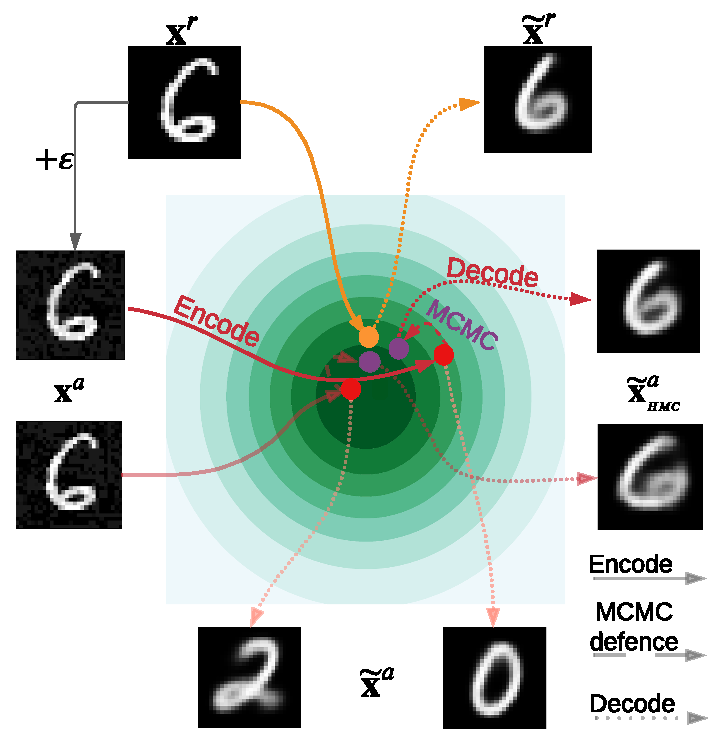
\includegraphics[width=0.6\linewidth]{pics/3_adv_att/Figure_1_upd.pdf}
		\caption{An example of an unsupervised encoder attack on VAE with 2D latent space and the proposed defense. 
			Given a single reference point $\rvx^r$ we learn additive perturbation $\varepsilon$, s.t. perturbed input $\rvx^a$ has the most different latent code and therefore the reconstruction $\widetilde{\rvx}^a$. 
			We observe that a single reference point can be mapped to extremely different regions of the latent space but using MCMC we are able to move them closer to the initial position so that the reconstruction $\widetilde{\rvx}^a_{\text{\tiny{HMC}}}$ is similar to the initial one $\widetilde{\rvx}^r$.}
		\label{fig:toy_exaple}
	\end{center}
\end{figure}
% \end{wrapfigure}

In this paper, we propose the method motivated by the following hypothesis: \textit{An adversarial attack maps the input to a latent region with a lower probability mass assigned by the true posterior (proportional to the conditional likelihood times the marginal over latents) and, eventually, we obtain incorrect reconstructions}. 
Therefore, a potential manner to alleviate the effect of an attack may rely on running a Markov chain to move the latent representation back to a more probable latent region. 
Such a defence is reasonable because we do not modify the training procedure or the model itself, we only insert a correction procedure. As a result, we propose to counteract adversarial attacks by enhancing the variational inference with Markov Chain Monte Carlo (MCMC) sampling. 
The illustrative example depicted in the Figure \ref{fig:toy_exaple} shows that the latent code of the adversarial input (red circle) moves closer to the latent code of the reference point (orange circle) after applying the MCMC (purple circle). 


The contribution of this work is the following:
\begin{itemize}%[leftmargin=*]
    \item We propose to use an MCMC technique during inference to correct adversarial attacks on VAEs.
    \item We show theoretically that the application of an MCMC technique could indeed help to counteract adversarial attacks (Theorem \ref{theorem:main}).
    \item We indicate empirically that the previously proposed strategies to counteract adversarial attacks do not generalize well across various datasets.
    \item We show empirically that the proposed approach (i.e., a VAE with an MCMC during inference) outperforms all baselines by a significant margin.
\end{itemize}

% In Figure \ref{fig:toy_exaple} we show an example of the \textit{supervised} attack on VAE with the 2D latent space. We show that we can add noise $\epsilon$ to a reference image so that the resulting adversarial input (second column) is encoded to a new point in the latent space. This new point is defined by the target image (first column). In \textit{unsupervised} attacks, on the other hand, we assume that the target image is not given. We show that it is still possible to construct an effective attack in this setting. The research goals of this work are the following:
% \begin{itemize}[leftmargin=*]
%     \item Defining robustness measures to understand how VAEs behave for adversarial attacks both in the latent space and the pixel space.
%     \item Assessing robustness of hierarchical and $\beta$-VAEs to adversarial attacks.
%     \item \jt{We need to add a bullet about MCMC to the rescue!}
% \end{itemize}


% %-------------------------------
% % ==== SECTION: Methodology ====
% %-------------------------------


% \section{Methodology}
\section{Background}

% ==== SubSECTION ====
\subsection{Variational Autoencoders}
Let us consider a vector of observable random variables, $\rvx \in \mathcal{X}^{D}$ (e.g., $\mathcal{X} = \mathbb{R}$) sampled from  the empirical distribution $p_{e}(\mathbf{\rvx})$, and vectors of latent variables $\rvz_{k} \in \mathbb{R}^{M_{k}}$, $k=1, 2, \ldots, K$, where $M_k$ is the dimensionality of each latent vector. First, we focus on a model with $K=1$ and the joint distribution $p_{\theta}(\rvx, \rvz) = \Dec{\rvx}{\rvz} p(\rvz)$. The marginal likelihood is then equal to $p_{\theta}(\rvx) = \int p_{\theta}(\rvx, \rvz) \mathrm{d} \rvz$. VAEs exploit variational inference \cite{jordan1999introduction} with a family of variational posteriors $\{\Enc{\rvz}{\rvx}\}$, also referred to as encoders, that results in a tractable objective function, i.e., the Evidence Lower BOund (ELBO): 
%$\mathcal{L}(\phi, \theta)
%    = \E_{p_{e}(\mathbf{\rvx})}\left( \E_{\Enc{\rvz}{\rvx}}\ln \Dec{\rvx}{\rvz} - \KL{\Enc{\rvz}{\rvx}}{p(\rvz)} \right)$. 
 \begin{align}
     \mathcal{L}(\phi, \theta)
     = \E_{p_{e}(\mathbf{\rvx})}\left( \E_{\Enc{\rvz}{\rvx}}\ln \Dec{\rvx}{\rvz} - \KL{\Enc{\rvz}{\rvx}}{p(\rvz)} \right).
 \end{align}

$\beta$-VAE \cite{higgins2016beta} uses a modified objective by weighting the $D_{\text{KL}}$ term by $\beta > 0$.
% \begin{equation}\label{eq:beta_elbo}
%     \mathcal{L}^{\beta}(\phi, \theta)
%     = \E_{p_{e}(\mathbf{\rvx})}\left( \E_{\Enc{\rvz}{\rvx}}\ln \Dec{\rvx}{\rvz} - \beta \KL{\Enc{\rvz}{\rvx}}{p(\rvz)} \right).
% \end{equation}
In the case of $K>1$, we consider a hierarchical latent structure with the generative model of the following form: 
\begin{equation}
    p_{\theta}(\rvx, \rvz_1, \ldots, \rvz_K) = \Dec{\rvx}{\rvz_1, \ldots, \rvz_K} \prod_{k=1}^{K}\Dec{\rvz_{k}}{\rvz_{>k}}.
\end{equation}
There are various possible formulations of the family of variational posteriors. However, here we follow the proposition of \citet{So_nderby2016-en} with the autoregressive inference model, namely, $$\Enc{\rvz_1, \ldots, \rvz_K}{\rvx} = \Enc{\rvz_K}{\rvx}\prod_{k=1}^{K-1}\HEnc{\rvz_k}{\rvz_{>k}, \rvx}.$$
This formulation was used, among others, in NVAE \citep{vahdat2020nvae}. Because of the top-down structure, it allows sharing data-dependent information between the inference model and the generative model.


% ==== SubSECTION ====
\subsection{Adversarial attacks}
\begin{table}[t]
	\caption[][\baselineskip]{Different types of attacks on the VAE. We denote $g_{\theta}(z)$ the deterministic mapping induced by decoder $p_{\theta}(x|z)$ and as $p_{\psi}(y|z)$ classification model in the latent space (downstream task).\\
		\textsuperscript{*} Only used during VAE training}
	\label{tab:attack_variation}
	\begin{center}
		\resizebox{\textwidth}{!}{
			% \begin{small}
			% \begin{sc}
			\begin{tabular}{llcccc}
				\toprule
				& \sc{Reference}  &$f(x)$ & $\Delta\left[A, B\right]$  &  $\|\cdot\|_p$ &  \sc{Type}\\ \midrule
				\multirow{3}{3cm}{Latent Space Attack}
				& \multirow{3}{2cm}{\cite{barrett2021certifiably, Gondim-Ribeiro2018-cu, Willetts2019-mu}}
				& \multirow{3}{*}{$q_{\phi}(\cdot|x)$} &  \multirow{3}{*}{$\KL{A}{B}$}   & \multirow{3}{*}{2} & \multirow{3}{*}{Supervised}\\
				&&&&&\\
				&&&&&\\
				\multirow{3}{3cm}{Unsupervised Encoder Attack}
				& \multirow{3}{2cm}{\cite{kuzina2021adv}}
				& \multirow{3}{*}{$q_{\phi}(\cdot|x)$} 
                    & \multirow{3}{*}{$\mathrm{SKL}\left[A\|B\right]$}   
                    & \multirow{3}{*}{2} 
                    & \multirow{3}{*}{Unsupervised}\\
				&&&&&\\
                    &&&&&\\
				\multirow{3}{3cm}{Targeted Output Attack}
				& \multirow{3}{*}{\cite{Gondim-Ribeiro2018-cu}}
				& \multirow{3}{*}{$g_{\theta}(\tilde{z}), \tilde{z} \sim q_{\phi}(\cdot|x)$}   
                    & \multirow{3}{*}{$\|A - B\|_2^2$}  
                    & \multirow{3}{*}{2} & \multirow{2}{*}{Supervised}\\
				&&&&&\\
                    &&&&&\\
				\multirow{3}{3cm}{Maximum Damage Attack}
				& \multirow{3}{2cm}{\cite{barrett2021certifiably, camuto2021towards}}
				& \multirow{3}{*}{$g_{\theta}(\tilde{z}), \tilde{z} \sim q_{\phi}(\cdot|x)$}   
                    & \multirow{3}{*}{$\|A - B\|_2^2$}  
                    & \multirow{3}{*}{2} 
                    & \multirow{3}{*}{Unsupervised}\\
				&&&&&\\
                    &&&&&\\
				\multirow{4}{3cm}{Projected Gradient Descent Attack\textsuperscript{*}}
				& \multirow{3}{*}{\cite{Cemgil2019-vn}}
				& \multirow{3}{*}{$q_{\phi}(\cdot|x)$} 
                    & \multirow{3}{*}{$\mathcal{WD}\left[A, B\right]$}   
                    & \multirow{3}{*}{$\inf$} 
                    & \multirow{3}{*}{Unsupervised}\\
				&&&&&\\
                    &&&&&\\
				\multirow{2}{3cm}{Adversarial Accuracy}
				& \multirow{2}{*}{\cite{cemgil2020autoencoding, Cemgil2019-vn}}
				& \multirow{2}{*}{$p_{\psi}(y|\tilde{z}), \tilde{z} \sim q_{\phi}(\cdot|x)$}  
                    & \multirow{2}{*}{\sc{Cross Entropy}} 
                    & \multirow{2}{*}{$\inf$} 
                    & \multirow{2}{*}{Unsupervised}\\
				&&&&&\\
				\bottomrule
		\end{tabular}}
		% \end{sc}
		% \end{small}
	\end{center}
	\vskip 15pt
\end{table}


\label{sect:adversarial_attacks}
An \textit{adversarial attack} is a slightly deformed data point that results in an undesired or unpredictable performance of a model \cite{goodfellow2014explaining}. In this work, we focus on the attacks that are constructed as an additive perturbation of the real data point $\rvx^r$ (which we will refer to as \textit{reference}), namely:
\begin{align}
    &\rvx^a = \rvx^r + \varepsilon, \text{where}\\
    &\|\varepsilon\|_{p} \leq \delta ,
\end{align}
where $\delta$ is the radius of the attack. The additive perturbation $\varepsilon$ is chosen in such a way that the attacked point does not differ from the reference point too much in a sense of a given similarity measure. It is a solution to an optimization problem solved by the attacker. The optimization problem could be formulated in various manners by optimizing different objectives and by having specific constraints and/or assumptions.

\paragraph{Attack construction} 
Let $f(x)$ be part of the model available to the attacker. In the case of VAEs, this, for example, may be an encoder network or an encoder with the downstream classifier in the latent space. The attacker uses a similarity measure $\Delta$ to learn an additive perturbation to a reference point. We consider two settings: \textit{unsupervised} and \textit{supervised}. In the former case, the perturbation is supposed to incur the largest possible change in $f$:
\begin{equation}\label{eq:objective_unsup}
    \varepsilon = \arg\max_{\|\varepsilon\|_p \leq \delta }\Delta\left[f(\rvx^r + \varepsilon) , f(\rvx^r) \right].
\end{equation}
The latter setting requires a \textit{target point} $\rvx^t$. The perturbation attempts to match the output for the target and the attacked points, namely:
\begin{equation}\label{eq:objective_sup}
    \varepsilon = \arg\min_{\|\varepsilon\|_p \leq \delta }\Delta\left[ f(\rvx^r + \varepsilon), f(\rvx^t) \right].
\end{equation}
There are different ways to select $f$ and $\Delta$ in the literature. Furthermore, different $L_p$-norms can be used to restrict the radius of the attack. Table \ref{tab:attack_variation} summarizes recent work on the topic. %adversarial attacks on VAE. 

In this work, we focus on attacking the encoder and the downstream classification task using unsupervised adversarial attacks. 
%\mw{I am slightly confused how the description below relates to the text above?}This work focuses on two types of unsupervised attacks\mw{isn't the second one a supervised attack?}: attack on the encoder and the downstream classification task. 
In the former, we maximize the symmetric KL-divergence to get the point with the most unexpected latent code and, therefore, the reconstruction. In the latter case, the latent code is passed to a classifier. The attack is trained to change the class of the point by maximizing the cross-entropy loss. However, the method we propose in Section \ref{sec:defence} is not limited to these setups since it is agnostic to how the attack was trained. 

%%%%%%%%%%%%%%%%%%%%
%-----SubSECTION-----
%%%%%%%%%%%%%%%%%%%%
\paragraph{Robustness measures} 
To measure the robustness of the VAE as well as the success of the proposed defence strategy, we focus on two metrics: $\mathrm{MSSSIM}$ and Adversarial accuracy.
For latent space attacks, we follow \citet{kuzina2021adv} in using Multi-Scale Structural Similarity Index Measure ($\mathrm{MSSSIM}$) \citep{wang2003multiscale}. We calculate $\mathrm{MSSSIM}[\widetilde{\rvx}^{r}, \widetilde{\rvx}^{a}]$, that is, the similarity between the reconstructions of $\rvx^{r}$ and the corresponding $\rvx^{a}$. We do not report the similarity between a reference and the corresponding adversarial input, since this value is the same for all the considered models (for a given attack radius). A successful adversarial attack would have a small value of  $\mathrm{MSSSIM}[\widetilde{\rvx}^{r}, \widetilde{\rvx}^{a}]$. 

For the attacks on the downstream classifier, we follow \citet{cemgil2020autoencoding, Cemgil2019-vn} and calculate the adversarial accuracy. For a given trained VAE model, we first train a linear classifier using latent codes as features. Afterwards, the attack is trained to fool the classifier. Adversarial accuracy is the proportion of points for which the attack was unsuccessful. Namely, when the predicted class of the reference and corresponding adversarial point are the same.  

%%%%%%%%%%%%%%%%%%%%
%-----SubSECTION-----
%%%%%%%%%%%%%%%%%%%%
\section{Preventing adversarial attacks with MCMC} \label{sec:defence}
% \subsection{Preventing adversarial attacks with MCMC}

\paragraph{Assumptions and the hypothesis}

We consider a scenario in which an attacker has access to the VAE encoder and, where relevant, to the downstream classification model. Above, we presented in detail how an attack could be performed. We assume that the defender cannot modify these components, but it is possible to add elements that the attacker has no access to. 

We hypothesize that \textit{the adversarial attacks result in incorrect reconstructions because the latent representation of the adversarial input lands in a region with a lower probability mass assigned by the true posterior. %being proportional to the conditional likelihood and the prior
}
This motivates us to use a method which brings the latents "back" to a highly probable region as a potential defence strategy. 
Since the adversarial attack destroys the input irreversibly, at the first sight it seems impossible to reconstruct the latent representation of the reference point. 
We aim at showing that this is possible to some degree theoretically and empirically (Appendix \ref{appendix:posterior_ratio}). 

\paragraph{The proposed solution } In order to steer the latents towards high probability regions, we propose to utilize an MCMC method during inference time. 
Since we are not allowed to modify the VAE or its learning procedure, this is a reasonable procedure from the defender's perspective. 
Another positive outcome of such an approach is that in a case of no attack, the latents given by the MCMC sampling will be closer to the mean of the posterior, thus, the reconstruction should be sharper or, at least, not worse. 
Note that the variational posterior approximates the true posterior from which the MCMC procedure samples. 
We propose to sample from $q^{(t)}(\rvz|\rvx) = \int Q^{(t)}(\rvz|\rvz_0) q_{\phi}(\rvz_0|\rvx) d\rvz_0$, where $Q^{(t)}(\rvz|\rvz_0)$ is a transition kernel of MCMC with $t$ steps and the target distribution $\pi(\rvz) = p_{\theta}(\rvz|\rvx) \propto p_{\theta}(\rvx|\rvz)p(\rvz)$. 
Alternatively, we can use optimization to find the mode of the posterior, however, MCMC can add extra benefits such as exploration of the typical set and randomness (see Appendix \ref{appendix:hmc_vs_opt} for details).

% Now, the naturally arising question is whether applying the MCMC could indeed help us in the case of an adversarial attack. 
To further analyze the proposed approach, we start with showing the following lemma:

\begin{lemma}\label{lemma:1}
Consider true posterior distributions of the latent code $\rvz$ for a data point $\rvx$ and its corrupted version $\rvx^a$.  
Assume also that $\ln p_{\theta}(\rvz|\rvx)$ is twice differentiable  over $\rvx$ with continuous derivatives at the neighbourhood around $\rvx=\rvx^r$. 
Then the KL-divergence between these two posteriors could be expressed using the small $o$ notation of the radius of the attack, namely:
% Consider true posterior distributions of the latent code $\rvz$ for a data point $\rvx^r$ and its corrupted version $\rvx^a$. Assume also that $\ln p_{\theta}(\rvz|\rvx)$ is differentiable at the point $\rvx = \rvx^r$. Then the KL-divergence between these two posteriors could be expressed using the small $o$ notation in terms of the radius of the attack, namely:
\begin{equation}
     \KL{ p_{\theta}(\rvz|\rvx^r)}{p_{\theta}(\rvz|\rvx^a)} = o(\|\varepsilon\|).
\end{equation}
\end{lemma}
\textit{Proof} See Appendix \ref{appendix:theory}.

According to Lemma \ref{lemma:1}, the difference (in the sense of the Kullback-Leibler divergence) between the true posteriors for a data point $\rvx$ and its corrupted version $\rvx^{a}$ decreases faster than the norm of the attack radius. However, it is important to note that this result is only valid for asymptotically small attack radius.

Next, the crucial step to show is whether we can quantify somehow the difference between the distribution over latents for $\rvx^a$ after running MCMC with $t$ steps, $q^{(t)}(\rvz|\rvx^a)$, and the variational distribution for $\rvx^r$, $q_{\phi}(\rvz|\rvx^r)$. 
We provide an important upper-bound for the Total Variation distance (TV)\footnote{The Total Variation fulfills the triangle inequality and it is a proper distance measure.} between $q^{(t)}(\rvz|\rvx^a)$ and $q_{\phi}(\rvz|\rvx^r)$ in the following lemma:

\begin{lemma}\label{lemma:2}
The Total Variation distance ($\mathrm{TV}$) between the variational posterior with MCMC for a given corrupted point $\rvx^a$, $q^{(t)}(\rvz|\rvx^a)$, and the variational posterior for a given data point $\rvx^r$, $q_{\phi}(\rvz|\rvx^r)$, can be upper bounded by the sum of the following three components:
\begin{align}
\TV{q^{(t)}(\rvz|\rvx^a)}{q_{\phi}(\rvz|\rvx^r)}
\leq &
    \TV{q^{(t)}(\rvz|\rvx^a)}{p_{\theta}(\rvz|\rvx^a)} \notag\\
    &+ 
    \sqrt{\tfrac12 \KL{ p_{\theta}(\rvz|\rvx^r)}{p_{\theta}(\rvz|\rvx^a)} } \notag\\
    &+
   \sqrt{\tfrac12  \KL{q_{\phi}(\rvz|\rvx^r)}{p_{\theta}(\rvz|\rvx^r)} }.
\end{align}
\end{lemma}
\textit{Proof} See Appendix \ref{appendix:theory}.

The difference expressed by $\TV{q^{(t)}(\rvz|\rvx^a)}{q_{\phi}(\rvz|\rvx^r)}$ is thus upper-bounded by the following three components:
\begin{itemize}
    \item The $\mathrm{TV}$ between  $q^{(t)}(\rvz|\rvx^a)$ and the real posterior for the corrupted image, $p_{\theta}(\rvz|\rvx^a)$. Theoretically, if $t \rightarrow \infty$, $q^{(\infty)}(\rvz|\rvx^a) = p_{\theta}(\rvz|\rvx^a)$ and, hence, $\TV{ q^{(\infty)}(\rvz|\rvx^a)}{p_{\theta}(\rvz|\rvx^a) } = 0$.
    \item The second component is the square root of the KL-divergence between the real posteriors for the image and its corrupted counterpart. Lemma \ref{lemma:1} gives us information about this quantity.
    \item The last element, the square root of $\KL{ q_{\phi}(\rvz|\rvx^r)}{p_{\theta}(\rvz|\rvx^r)}$, quantifies the \textit{approximation gap} \cite{cremer2018inference}, i.e., the difference between the best variational posterior from a chosen family, and the true posterior. This quantity has no direct connection with adversarial attacks. However, as we can see, using a rich family of variational posteriors can help us to obtain a tighter upper-bound. In other words, taking flexible variational posteriors allows to counteract attacks. This finding is in line with the papers that propose to use hierarchical VAEs as the means for preventing adversarial attacks \cite{Willetts2019-mu}.
\end{itemize}

Eventually, by applying Lemma \ref{lemma:1} to Lemma \ref{lemma:2}, we obtain the following result:

\begin{theorem}\label{theorem:main}
The upper bound on the total variation distance between samples from MCMC for a given corrupted point $\rvx^a$, $q^{(t)}(\rvz|\rvx^a)$, and the variational posterior for the given real point $\rvx^r$, $q_{\phi}(\rvz|\rvx^r)$, is the following:
\begin{align} \label{eq:theorem_1_main}
    \TV{ q^{(t)}(\rvz|\rvx^a)}{q_{\phi}(\rvz|\rvx^r) }
\leq 
&  \,\TV{ q^{(t)}(\rvz|\rvx^a)}{p_{\theta}(\rvz|\rvx^a) } \notag \\
    &+ 
   \sqrt{\tfrac12  \KL{ q_{\phi}(\rvz|\rvx^r) }{ p_{\theta}(\rvz|\rvx^r)} } \notag\\
   &+ o(\sqrt{\|\varepsilon\|}).
%   \xrightarrow{t\rightarrow \inf}  
%   \sqrt{\tfrac12  \text{KL}\left[ q_{\phi}(\rvz|\rvx) \| p_{\theta}(\rvz|\rvx)\right]} + o(\|\varepsilon\|)
\end{align}
\end{theorem}
\textit{Proof} See Appendix \ref{appendix:theory}.


As discussed already, the first component gets smaller with more steps of the MCMC. %In other words, we can say that it results in the \mw{not so sure this is only variance, as during burn in we also have bias} \textit{variance} (the more steps of the MCMC we apply, the smaller the difference). 
The second component could be treated as a \textit{bias} of the family of variational posteriors. Finally, there is the last element that corresponds to a constant error that is unavoidable. However, this term decays faster than the square root of the attack radius for the asymptotically small attack radius.

\paragraph{Specific implementation of the proposed approach}
In this paper, we use a specific MCMC method, namely, the Hamiltonian Monte Carlo (HMC) \cite{betancourt2017conceptual, duane1987hybrid}. Once the VAE is trained, the attacker calculates an adversarial point $\rvx^a$ using the encoder of the VAE. After the attack, the latent representation of $\rvx^a$ is calculated, $\rvz^a$, and used as the initialization of the HMC.

In the HMC, the target (unnormalized) distribution is $p(\mathbf{x}^{a}|\mathbf{z}) p(\mathbf{z})$. The Hamiltonian is then the energy of the joint distribution of $\rvz$ and the auxilary variable $\rvp$, that is:
\begin{align}
    H(\rvz, \rvp) &= U(\rvz) + K(\rvp),\\
    U(\rvz) &= - \ln p_{\theta}(\mathbf{x}^{a}|\mathbf{z}) - \ln p(\mathbf{z}),\\
    K(\rvp) &= -\tfrac12 \rvp^T\rvp.
\end{align}
When applying the proposed defence to hierarchical models, we update all the latent variables simultaneously. That is, we have $\rvz = \{ \rvz_1, \dots, \rvz_K\}$ and
% \begin{equation}
$U(\rvz) = -\ln \Dec{\rvx^a}{\rvz} - \sum_{k=1}^K\ln p_{\theta}(\rvz_k|\rvz_{k+1}). $
% \end{equation}


\begin{algorithm}
	\caption{One Step of HMC.}
	\label{alg:hmc_step}
	\begin{algorithmic} %[1]
 \\\hrulefill
	   \State \hskip-3mm \textbf{Input}: $\rvz, \eta, L$
		\State $\rvp \sim \mathcal{N}(0,I)$. \Comment{Sample the auxiliary variable }
		\State $\rvz^{(0)} := \rvz, \rvp^{(0)}:=\rvp$.
		\For{$l = 1 \dots, L$} \Comment{Make $L$ steps of \textit{leapfrog}.}
        \State $ \rvp^{(l)} = \rvp^{(l-1)} - \frac{\eta}{2}\nabla_{\rvz} U(\mathbf{z}^{(l)})$.
		\State $\rvz^{(l)} = \rvz^{(l)} + \eta  \nabla_{\rvp} K(\rvp^{(l)})$.
		\State $\rvp^{(l)} = \rvp^{(l)} - \frac{\eta}{2}\nabla_{\rvz} U(\mathbf{z}^{(l)})$.
		\EndFor
		\State $\alpha = \min\left(1, \exp\left(- H(\rvz^{(L)}, \rvp^{(L)}) + H(\rvz^{(0)}, \rvp^{(0)})\right) \right)$
		\State $\rvz =
\begin{cases}
\rvz^{(L)}\, \text{with probability}\, \alpha ,\\
\rvz^{(0)}\, \text{otherwise}.
\end{cases}$  \Comment{Accept a new point with prob. $\alpha$.}
        \State  \hskip-3mm \textbf{Return}: $\rvz$
	\end{algorithmic}
\end{algorithm}

Eventually, the resulting latents from the HMC are decoded. The steps of the whole process are presented below:
\begin{enumerate}%[wide, labelwidth=0pt, labelindent=0pt]
    \item (\textit{Defender}) Train a VAE: $q_{\phi}(\rvz|\rvx)$, $p(\rvz)$, $p_{\theta}(\rvx|\rvz)$.
    \item (\textit{Attacker}) For given $\rvx^r$, calculate the attack $\rvx^{a}$ using the criterion from Eq.~\ref{eq:objective_unsup} or Eq.~\ref{eq:objective_sup}.
    \item (\textit{Defender}) Initialize the latent code $\rvz := \rvz_0$, where $\rvz_{0} \sim q_{\phi}(\rvz|\rvx^{a})$. Then, run $T$ steps of HMC (Algorithm \ref{alg:hmc_step}) with the step size $\eta$ and $L$ \textit{leapfrog} steps.
\end{enumerate}

The resulting latent code $\rvz$ can be passed to the decoder to get a reconstruction or to the downstream classification task.



% %-------------------------------
% % ==== SECTION: Experiments ====
% %-------------------------------

% \newpage
\section{Experiments} \label{sec:experiments}
\subsection{Posterior ratio}\label{sec:exp_ratio}

%\begin{wrapfigure}{r}{0.55\textwidth}
%    \centering
%        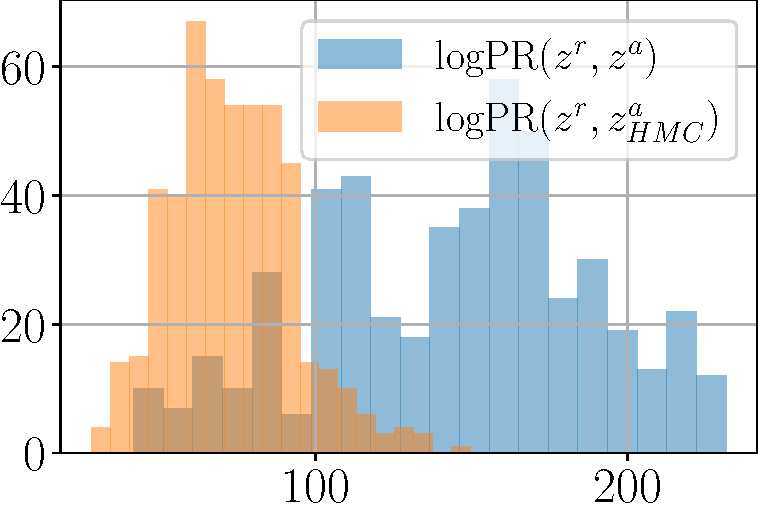
\includegraphics[width=0.45\textwidth]{pics/3_adv_att/mnist_posterior_ratio.pdf}
%    \caption{Histograms of the log posterior ratios \textcolor{blue}{before HMC (blue)} and \textcolor{orange}{after HMC (orange)} evaluated on the MNIST dataset.}
%    \label{fig:mnist_post_ratio_main}
%\end{wrapfigure}
\begin{figure}
	\centering
	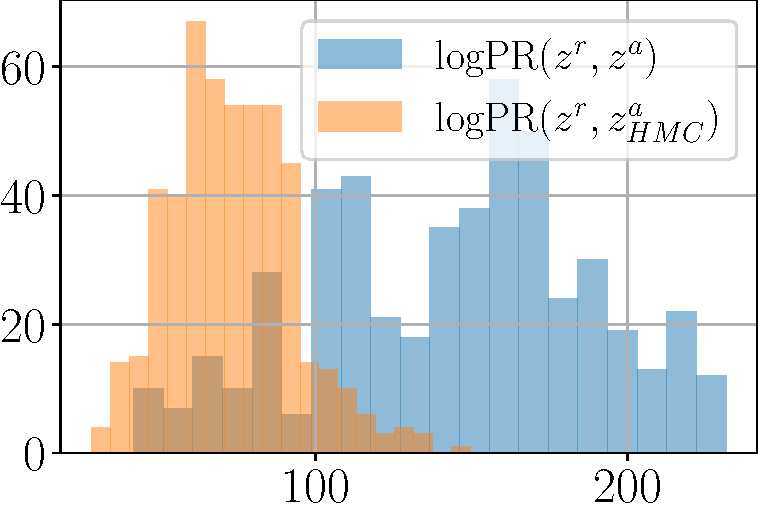
\includegraphics[width=0.5\textwidth]{pics/3_adv_att/mnist_posterior_ratio.pdf}
	\caption{Histograms of the log posterior ratios \textcolor{blue}{before HMC (blue)} and \textcolor{orange}{after HMC (orange)} evaluated on the MNIST dataset.}
	\label{fig:mnist_post_ratio_main}
\end{figure}

We motivate our method by the hypothesis that the adversarial attack "shifts" a latent code to the region of a lower posterior density, while our approach moves it back to a high posterior probability region. In Section \ref{sec:defence} we theoretically justify our hypothesis, while here we provide an additional empirical evidence.
% In order to verify our claim that applying an MCMC method allows us to counteract attacks by moving a latent code from a region of a lower posterior probability mass to a region of a higher density, we propose to quantify this effect by measuring the ratio of posteriors for $\rvz_1$ and $\rvz_2$. 
The true posterior $p(\rvz | \rvx^{r})$ is not available due to the cumbersome marginal distribution $p(\rvx^{r})$, however, we can calculate the ratio of posteriors because the marginal will cancel out. In our case, we are interested in calculating the posterior ratio between the reference and adversarial latent codes ($\rvz_1 = \rvz^r$,  $\rvz_2 = \rvz^a$) as the baseline, and the posterior ratio between the reference and adversarial code after applying the HMC ($\rvz_1 = \rvz^r$ , $\rvz_2 = \rvz^a_{\text{HMC}}$). The lower the posterior ratio, the better. For practical reasons, we use the logarithm of the posterior ratio since the logarithm does not change the monotonicity and turns products to sums:
\begin{equation}
    \log \text{PR}(\rvz_1, \rvz_2) = \log p_{\theta}(\rvx^r|\rvz_1) + \log p(\rvz_1) - \log p_{\theta}(\rvx^r| \rvz_2) - \log p(\rvz_2) .
\end{equation}
% , namely:

% \begin{align}
% \text{PR}(\rvz_1, \rvz_2) &= \tfrac{p_{\theta}(\rvz_1|\rvx^r)}{p_{\theta}(\rvz_2|\rvx^r)} \\
% &= \tfrac{p_{\theta}(\rvx^r|\rvz_1)p(\rvz_1)}{p_{\theta}(\rvx^r| \rvz_2)p(\rvz_2)} .
% \end{align}
In Figure \ref{fig:mnist_post_ratio_main} we show a plot with two histograms: one with the posterior ratio between the reference and adversarial latent codes ($\rvz_1 = \rvz^r$,  $\rvz_2 = \rvz^a$) in blue, and the second histogram of the posterior ratio between the reference and adversarial code after applying the HMC ($\rvz_1 = \rvz^r$ , $\rvz_2 = \rvz^a_{\text{HMC}}$) in orange. We observe that the histogram has moved to the left after applying the HMC. This indicates that posterior of the adversarial (in the denominator) is increasing when the HMC is used. This is precisely the effect we hoped for and this result provides an empirical evidence in favor of our hypothesis. For more details see \ref{appendix:posterior_ratio}.


% \mw{Max: corrected until here}
% In this section, we experimentally evaluate performance of the proposed approach 
% % \footnote{Our code is publicly available at \url{hidden-repository-due-to-double-blind-review}.}. 
% We perform experiments on a variety of VAE models ($\beta$-VAE, $\beta$-TCVAE and NVAE) and datasets (MNIST. Fashion MNIST, Color MNIST, CelebA).

% ==== SubSECTION ====
\subsection{VAE, $\beta$-VAE and $\beta$-TCVAE} %\texorpdfstring{
% First, we consider attacks on VAE with a single level of latent variables. 
All implementation details and hyperparameters are included in the Appendix ~\ref{appendix:experimental_details} and code repository~\footnote{\url{github.com/AKuzina/defend_vae_mcmc}}. 
\paragraph{Datasets}
VAEs are trained on the MNIST, Fashion MNIST \cite{xiao2017fashion} and Color MNIST datasets. Following \cite{Cemgil2019-vn}, we construct the Color MNIST dataset from MNIST by artificially coloring each image with seven colors (all corners of RGB cube except for black). 

% \begin{wrapfigure}{r}{0.55\textwidth}
\begin{figure}
%\vskip -5pt
    \centering
    \begin{tabular}{ccccc}
        
\includegraphics[width=0.1\linewidth]{pics/3_adv_att/mnist_ref_4.pdf} & 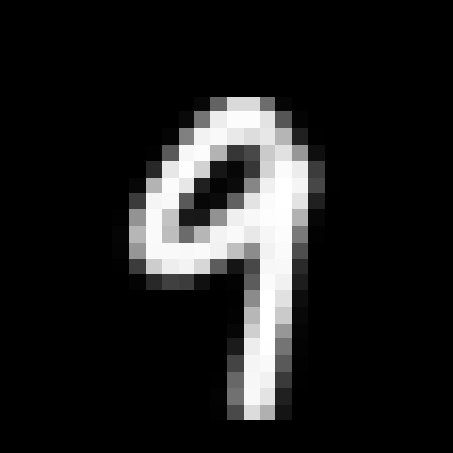
\includegraphics[width=0.1\linewidth]{pics/3_adv_att/mnist_ref_rec_4.pdf} &
        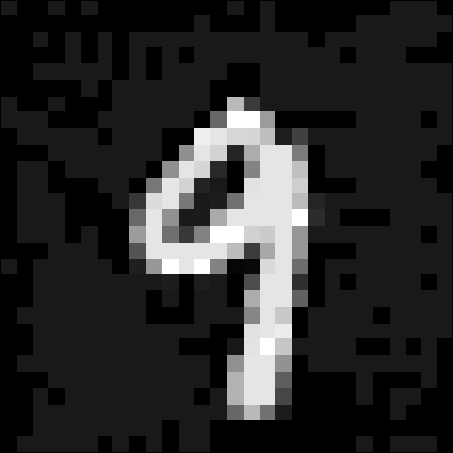
\includegraphics[width=0.1\linewidth]{pics/3_adv_att/mnist_adv_4.pdf} & 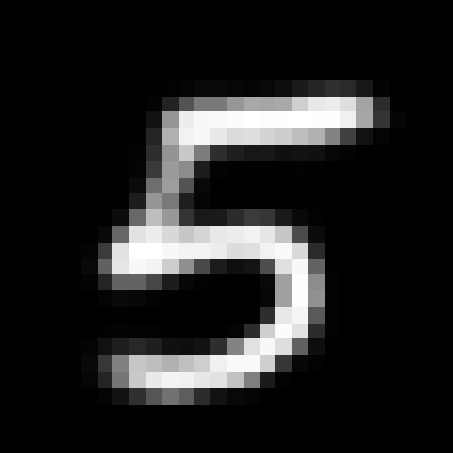
\includegraphics[width=0.1\linewidth]{pics/3_adv_att/mnist_adv_rec_4.pdf} & 
        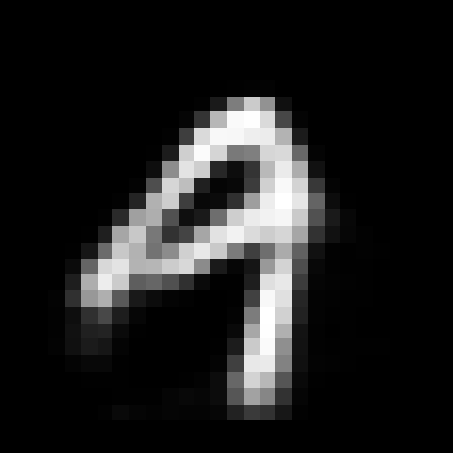
\includegraphics[width=0.1\linewidth]{pics/3_adv_att/mnist_adv_rec_hmc_4.pdf}\\
        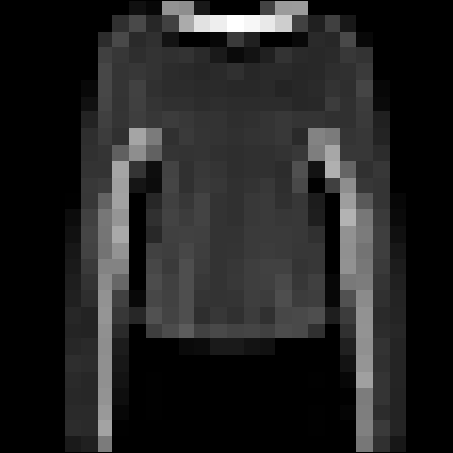
\includegraphics[width=0.1\linewidth]{pics/3_adv_att/fashion_mnist_ref_14.pdf} & 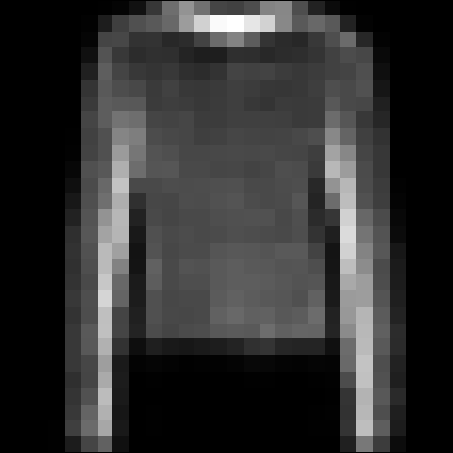
\includegraphics[width=0.1\linewidth]{pics/3_adv_att/fashion_mnist_ref_rec_14.pdf} &
        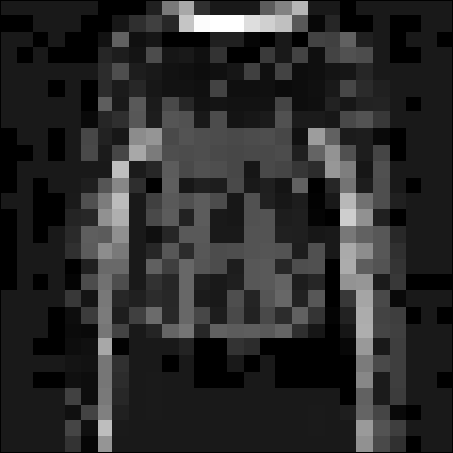
\includegraphics[width=0.1\linewidth]{pics/3_adv_att/fashion_mnist_adv_14.pdf} & 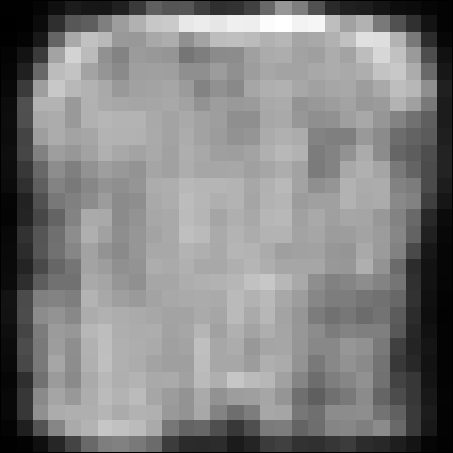
\includegraphics[width=0.1\linewidth]{pics/3_adv_att/fashion_mnist_adv_rec_14.pdf} & 
        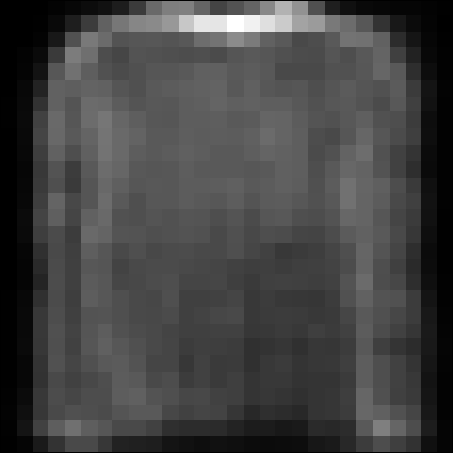
\includegraphics[width=0.1\linewidth]{pics/3_adv_att/fashion_mnist_adv_rec_hmc_14.pdf}\\
        
\includegraphics[width=0.1\linewidth]{pics/3_adv_att/color_mnist_ref_4.pdf} & 
\includegraphics[width=0.1\linewidth]{pics/3_adv_att/color_mnist_ref_rec_4.pdf} &
        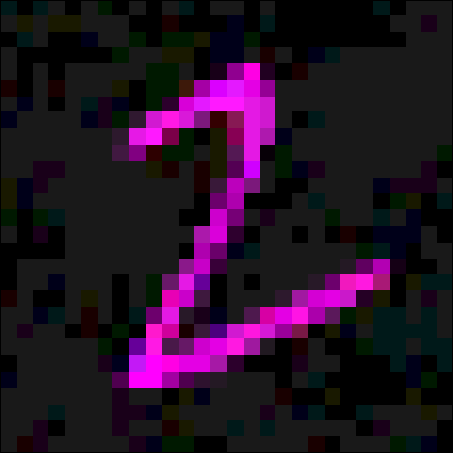
\includegraphics[width=0.1\linewidth]{pics/3_adv_att/color_mnist_adv_4.pdf} & 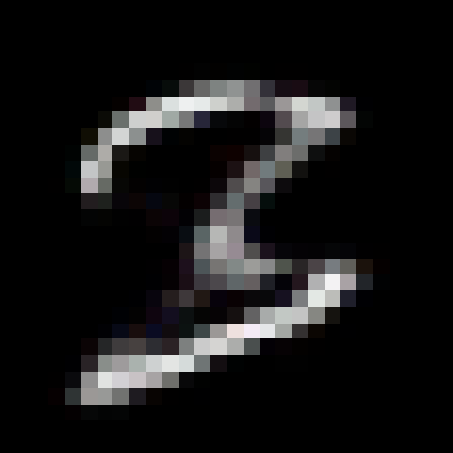
\includegraphics[width=0.1\linewidth]{pics/3_adv_att/color_mnist_adv_rec_4.pdf} & 
        
\includegraphics[width=0.1\linewidth]{pics/3_adv_att/color_mnist_adv_rec_hmc_4.pdf}\\
        
\includegraphics[width=0.1\linewidth]{pics/3_adv_att/color_mnist_ref_9.pdf} & 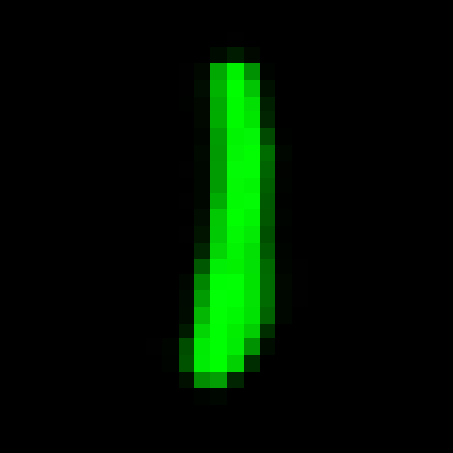
\includegraphics[width=0.1\linewidth]{pics/3_adv_att/color_mnist_ref_rec_9.pdf} &
        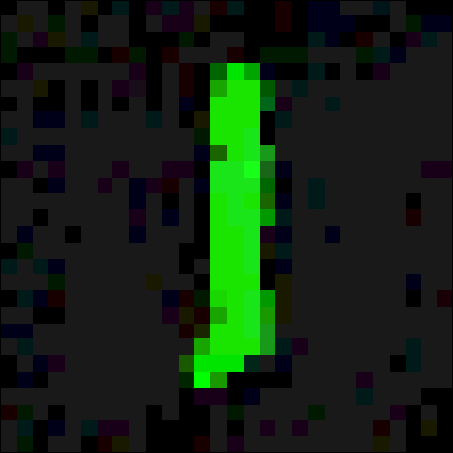
\includegraphics[width=0.1\linewidth]{pics/3_adv_att/color_mnist_adv_9.pdf} & 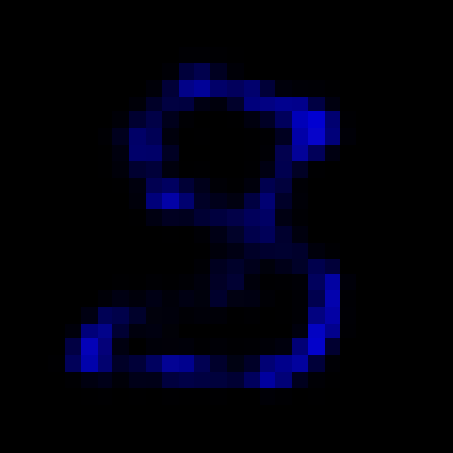
\includegraphics[width=0.1\linewidth]{pics/3_adv_att/color_mnist_adv_rec_9.pdf} & 
        
\includegraphics[width=0.1\linewidth]{pics/3_adv_att/color_mnist_adv_rec_hmc_9.pdf}\\
        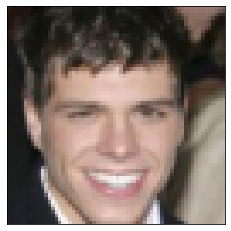
\includegraphics[width=0.1\linewidth]{pics/3_adv_att/celeba_ref_1.png} & 
\includegraphics[width=0.1\linewidth]{pics/3_adv_att/celeba_ref_rec_1.png} &
        
\includegraphics[width=0.1\linewidth]{pics/3_adv_att/celeba_adv_1.png} & 
\includegraphics[width=0.1\linewidth]{pics/3_adv_att/celeba_adv_rec_1.png} & 
        
\includegraphics[width=0.1\linewidth]{pics/3_adv_att/celeba_adv_rec_hmc_1.png}\\
        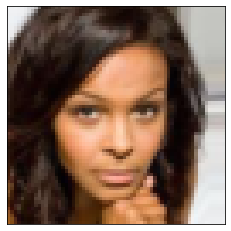
\includegraphics[width=0.1\linewidth]{pics/3_adv_att/celeba_ref_2.png} & 
\includegraphics[width=0.1\linewidth]{pics/3_adv_att/celeba_ref_rec_2.png} &
        
\includegraphics[width=0.1\linewidth]{pics/3_adv_att/celeba_adv_2.png} & 
\includegraphics[width=0.1\linewidth]{pics/3_adv_att/celeba_adv_rec_2.png} & 
        
\includegraphics[width=0.1\linewidth]{pics/3_adv_att/celeba_adv_rec_hmc_2.png}\\
        (a) $\rvx^r$ & (b) $\widetilde{\rvx}^r$ & (c) $\rvx^a$ & (d) $\widetilde{\rvx}^a$ & (e) $\widetilde{\rvx}^\text{a}_{\text{HMC}}$ \\
    \end{tabular}
    \caption{Examples of (a) reference points, (b) reconstructions of the reference points, (c) adversarial points, (d) reconstructions of the adversarial points, (e) reconstructions of the adversarial points after the proposed defence (HMC). All the adversarial examples are unsupervised attacks on the encoder. Last two rows contain examples for the NVAE model discussed in Section \protect\ref{sec:nvae}}
    \label{fig:adversarial_examples}
    \vspace*{\baselineskip}
\end{figure}
% \end{wrapfigure}


\paragraph{Models}
We train vanilla fully convolutional VAEs, as well as $\beta$-VAE \cite{higgins2016beta} and $\beta$-TCVAE \cite{chen2018isolating, kim2018disentangling}. Both $\beta$-VAE and $\beta$-TCVAE modify the ELBO objective to encourage disentanglement. $\beta$-VAE weighs the KL-term in the ELBO with $\beta > 0$. It is said that the larger values of $\beta$ encourage disentangling of latent representations \cite{chen2018isolating} and improve the model robustness as observed by \cite{camuto2021towards}. $\beta$-TCVAE puts a higher weight on the total correlation (TC) term of the ELBO. Penalization of the total correlation was shown to increase the robustness of VAE adversarial attacks \cite{Willetts2019-mu}.

In Appendix \ref{appendix:beta_vae_param} we provide details of the architecture, optimization, and results on the test dataset for VAE trained with different values of $\beta$. 
We note that the optimal value in terms of the negative log-likelihood (NLL) is always $\beta=1$. Larger values of $\beta$ are supposed to improve robustness in exchange for the reconstruction quality. When evaluating the robustness of $\beta$-VAE and $\beta$-TCVAE, we train models with $\beta \in \{2, 5, 10\}$. Then, we select the value of $\beta$ that provides the most robust model in terms of the used metric. Next, we apply our defence strategy to this model to observe the potential performance improvement. 


\begin{table}[h]
\caption[][\baselineskip]{Results for unsupervised attack with radius $0.1$ and $0.2$ on MNIST and Fashion MNIST datasets. We attack the encoder (left) and the downstream classification task (right).
% Higher values correspond to more robust models.
\\\textsuperscript{$\dagger$} Our implementation.}
\vskip -0.2cm
\label{tab:mnist_attack_result}
\begin{center}
\begin{small}
\begin{sc}
\resizebox{1.0\textwidth}{!}{
\begin{tabular}{lllcc|ccc|ll}
\toprule
& & & \multicolumn{2}{c|}{$\mathrm{MSSSIM}[\widetilde{\rvx}^{r}, \widetilde{\rvx}^{a}]$ $\uparrow$} & \multicolumn{3}{c|}{Adversarial Accuracy $\uparrow$} & \multirow{2}{*}{MSE $\downarrow$}  \\
\multicolumn{3}{c}{$\|\varepsilon\|$} & 0.1 & 0.2 & 0.0 & 0.1 & 0.2           & &\\ 
\midrule
 & \multirow{3}{*}{\STAB{\rotatebox[origin=c]{90}{\small{MNIST}}}} 
 & VAE & 0.70 \tiny{(0.02)} & 0.36 \tiny{(0.03)} & \textbf{0.90} \tiny{(0.04)} & 0.08 \tiny{(0.04)} & 0.05 \tiny{(0.03)} & 578.7 \\
&& \textbf{VAE + HMC} & \textbf{0.88} \tiny{(0.01)} & \textbf{0.76} \tiny{(0.02)} & 0.76 \tiny{(0.01)} & \textbf{0.25} \tiny{(0.03)} & \textbf{0.19} \tiny{(0.03)} & \textbf{478.1} 
\\
&& $\beta$-VAE & 0.75 \tiny{(0.01)} & 0.50 \tiny{(0.03)} & 0.90 \tiny{(0.05)} & 0.11 \tiny{(0.04)} & 0.01 \tiny{(0.01)} & 824.2 \\
&& $\beta$-TCVAE\textsuperscript{$\dagger$} 
& 0.70 \tiny{(0.02)} & 0.46 \tiny{(0.03)} & 0.86 \tiny{(0.05)} & 0.05 \tiny{(0.03)} & 0.03 \tiny{(0.02)} & 828.4
\\ \midrule 
\multirow{3}{*}{\STAB{\rotatebox[origin=c]{90}{\small{Fashion}}}} &\multirow{3}{*}{\STAB{\rotatebox[origin=c]{90}{\small{MNIST}}}} 
&VAE           & 0.59 \tiny{(0.03)} & 0.47 \tiny{(0.03)} & 0.78 \tiny{(0.06)} & 0.00 \tiny{(0.01)} & 0.01 \tiny{(0.01)} & 814.2  \\
&& \textbf{VAE + HMC}    & \textbf{0.66} \tiny{(0.03)} & \textbf{0.54} \tiny{(0.03)} & 0.56 \tiny{(0.01)} & \textbf{0.14} \tiny{(0.02)} & \textbf{0.13} \tiny{(0.02)} & \textbf{764.2} \\ 
&& $\beta$-VAE & 0.52 \tiny{(0.03)} & 0.41 \tiny{(0.03)} & 0.80 \tiny{(0.05)} & 0.00 \tiny{(0.01)} & 0.00 \tiny{(0.01)} & 
1021.1\\
&& $\beta$-TCVAE\textsuperscript{$\dagger$} & 0.52 \tiny{(0.03)} & 0.42 \tiny{(0.03)} & \textbf{0.84} \tiny{(0.05)} & 0.00 \tiny{(0.01)} & 0.02 \tiny{(0.02)} & 980.4\\ 
\bottomrule
\end{tabular}
}
\end{sc}
\end{small}
\end{center}
\vspace*{\baselineskip}
\end{table}

%%%% MOVED TO APPENDIX
% \begin{figure}[t]
%     \centering
%     \begin{tabular}{ll}
%         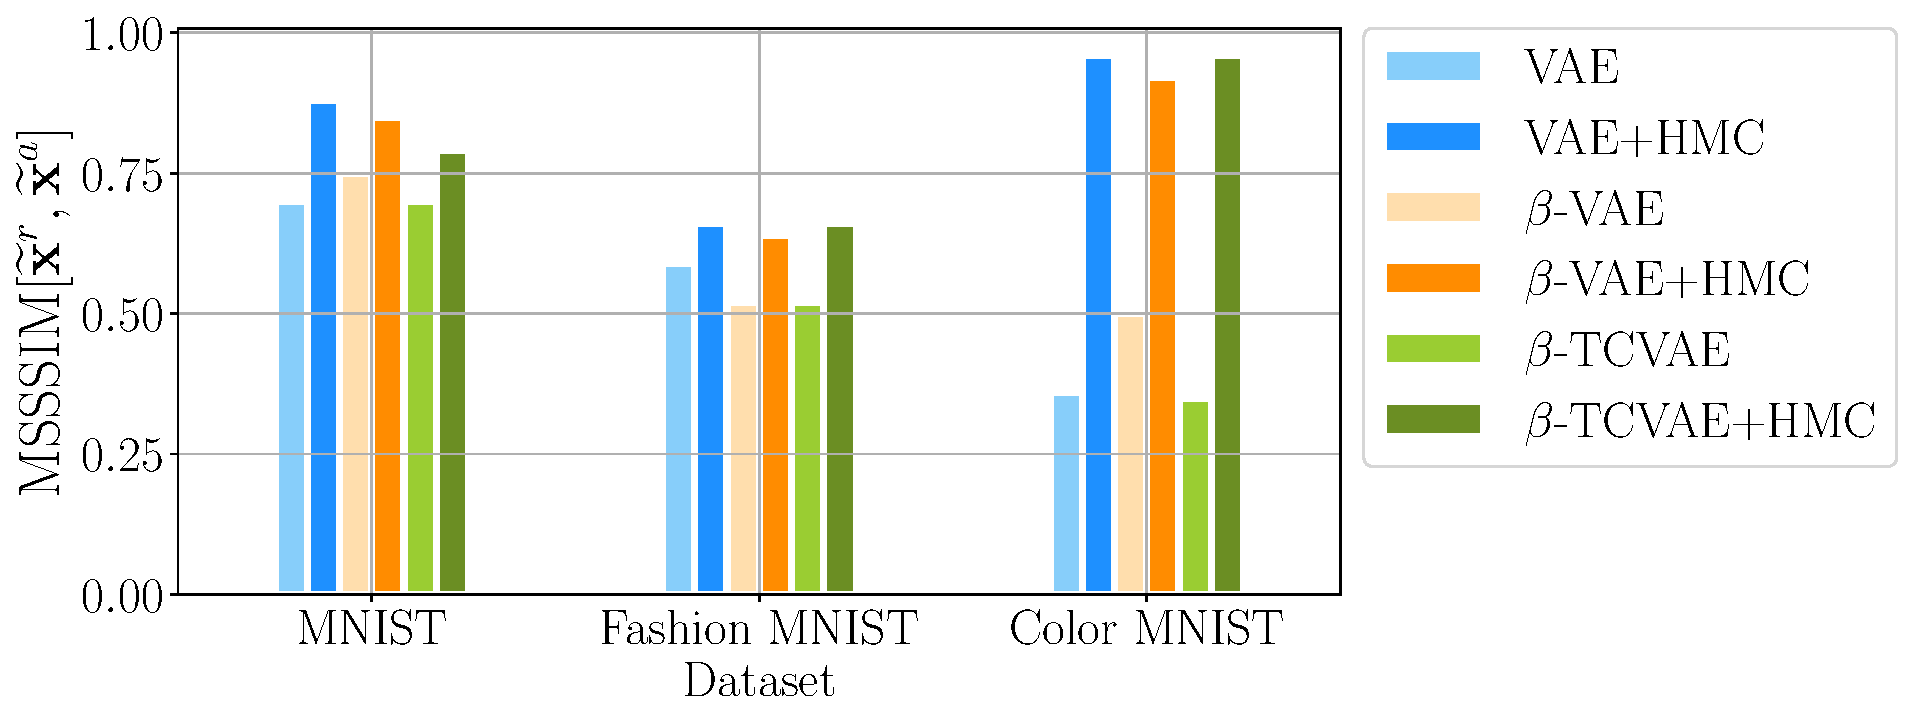
\includegraphics[width=0.5\textwidth]{img/msssim_eps_1.pdf} & 
%         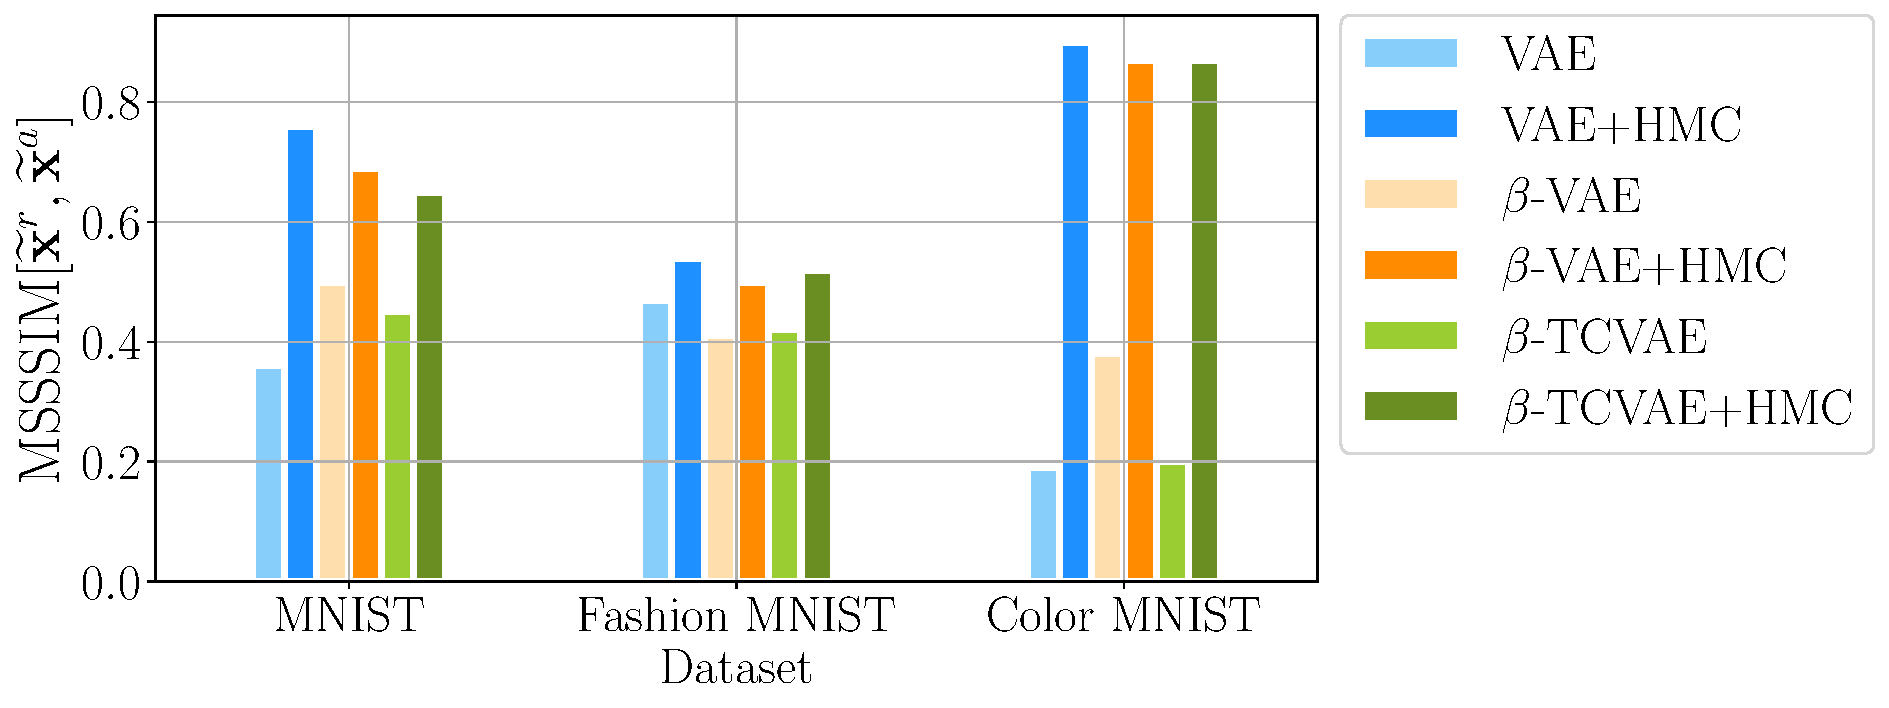
\includegraphics[width=0.5\textwidth]{img/msssim_eps_2.pdf} \\
%         \multicolumn{1}{c}{(a) $||\varepsilon ||_{\inf} = 0.1$} &
%         \multicolumn{1}{c}{(b) $||\varepsilon ||_{\inf} = 0.2$} \\
%         % (a) & (b) \\
%         % (c) & (d)
%     \end{tabular}
%     \caption{Improvement of the Reconstruction Similarity after the proposed defence. We fix the attack radius to be equal to (a) 0.1 and (b) 0.2. Higher values correspond to a more robust representations.}
%     \vskip -10pt
%     \label{fig:mnist_rec_similarity}
% \end{figure}


\begin{table}[ht]
\caption[][\baselineskip]{Results for unsupervised attack with radius $0.1$ and $0.2$ on ColorMNIST dataset. We attack the encoder (left) and the downstream classification task (right).
% Higher values correspond to more robust models.
\\ \textsuperscript{$\dagger$} Our implementation. \\
\textsuperscript{*} Values reported in \cite{cemgil2020autoencoding}, VAE implementation and evaluation protocol may differ. }
\vskip -0.2cm
\label{tab:color_mnist_attack_results}
\begin{center}
\begin{small}
\begin{sc}
\resizebox{1.03\textwidth}{!}{
\begin{tabular}{lcc|cccccc|ll}
\toprule
 & \multicolumn{2}{c|}{$\mathrm{MSSSIM}[\widetilde{\rvx}^{r}, \widetilde{\rvx}^{a}]$ $\uparrow$} & \multicolumn{6}{c|}{Adversarial Accuracy $\uparrow$} & \multirow{3}{*}{MSE$\downarrow$} &  \multirow{3}{*}{FID $\downarrow$} \\
 &     &     & \multicolumn{3}{c}{Digit} &  \multicolumn{3}{c|}{Color} & & \\
 $\|\varepsilon\|$& 0.1 & 0.2 & 0.0 & 0.1 & 0.2           & 0.0 & 0.1 & 0.2             & & \\ \midrule
% \multirow{9}{*}{\STAB{\rotatebox[origin=c]{90}{Color MNIST}}} & 
VAE & 0.36 \tiny{(0.03)} & 0.19 \tiny{(0.02)} & \textbf{1.00 \tiny{(0.00)}} & 0.04 \tiny{(0.03)} & 0.02 \tiny{(0.02)} & 1.00 \tiny{(0.00)} & 0.06 \tiny{(0.03)} & 0.06 \tiny{(0.03)} & \textbf{261} & \textbf{2.1}\\
% & 
\textbf{VAE + HMC}
& \textbf{0.96 \tiny{(0.01)}} & \textbf{0.90 \tiny{(0.01)}} & 0.42 \tiny{(0.01)} & 0.16 \tiny{(0.02)} & 0.11 \tiny{(0.02)} & 1.00 \tiny{(0.00)} & 0.68 \tiny{(0.03)} & 0.62 \tiny{(0.03)} & \textbf{206} & \textbf{2.1}\\
\midrule
$\beta$-VAE 
& 
0.75 \tiny{(0.01)} & 0.5 \tiny{(0.03)} & 0.88 \tiny{(0.04)} & 0.08 \tiny{(0.04)} & 0.05 \tiny{(0.03)} & 1.00 \tiny{(0.00)} & 0.21 \tiny{(0.06)} & 0.18 \tiny{(0.05)} & 366 & 2.4\\
$\beta$-TCVAE\textsuperscript{$\dagger$} 
& 
0.35 \tiny{(0.02)} & 0.23 \tiny{(0.02)} & 0.94 \tiny{(0.04)} & 0.08 \tiny{(0.04)} & 0.05 \tiny{(0.03)} & 1.00 \tiny{(0.00)} & 0.06 \tiny{(0.03)} & 0.05 \tiny{(0.02)} & 366 & 3.0\\
% & 
$\text{SE}_{0.1}$\textsuperscript{*}
& N/A                & N/A                & 0.94 \tiny{(N/A)}  & 0.89 \tiny{(N/A)}  & 0.02 \tiny{(N/A)}  & 1.00 \tiny{(N/A)}  & 1.00 \tiny{(N/A)}  & 0.22 \tiny{(N/A)}  & 1372 & 13.0\\
% & 
$\text{SE}_{0.2}$\textsuperscript{*}
& N/A                & N/A                & 0.95 \tiny{(N/A)}  & 0.92 \tiny{(N/A)}  & \textbf{0.87 \tiny{(N/A)}}  & 1.00 \tiny{(N/A)}  & 1.00 \tiny{(N/A)}  & \textbf{1.00 \tiny{(N/A)}}  & 1375 & 11.7 \\
% & 
AVAE\textsuperscript{*} 
& N/A                & N/A                & 0.97 \tiny{(N/A)}  & 0.88 \tiny{(N/A)}  & 0.55 \tiny{(N/A)}  & 1.00 \tiny{(N/A)}  & 1.00 \tiny{(N/A)} & 0.88 \tiny{(N/A)}  & 1372 & 15.5\\
% & 
$\text{SE}_{0.1}$-AVAE\textsuperscript{*}
& N/A                & N/A                & 0.97 \tiny{(N/A)}  & \textbf{0.94 \tiny{(N/A)}}  & 0.25 \tiny{(N/A)}  & 1.00 \tiny{(N/A)}  & 1.00 \tiny{(N/A)}  & 0.60 \tiny{(N/A)}  & 1373 & 13.9\\
% & 
$\text{SE}_{0.2}$-AVAE\textsuperscript{*} 
& N/A                & N/A                & 0.98 \tiny{(N/A)}  & \textbf{0.94 \tiny{(N/A)}}  & 0.80 \tiny{(N/A)}  & 1.00 \tiny{(N/A)}  & 1.00 \tiny{(N/A)}  & 0.83 \tiny{(N/A)}  & 1374 & 13.9\\
% & 
AVAE-SS\textsuperscript{*} 
& N/A                & N/A                & 0.94 \tiny{(N/A)}  & 0.73 \tiny{(N/A)}  & 0.21 \tiny{(N/A)}  & 1.00 \tiny{(N/A)}  & 1.00 \tiny{(N/A)}  & 0.57 \tiny{(N/A)}  & 1379 & 12.4\\
\bottomrule
\end{tabular}}
\end{sc}
\end{small}
\end{center}
\vspace*{\baselineskip}
\end{table}

%%%% MOVED TO APPENDIX
% \begin{figure}[t]
%     \centering
%     \begin{tabular}{ll}
%         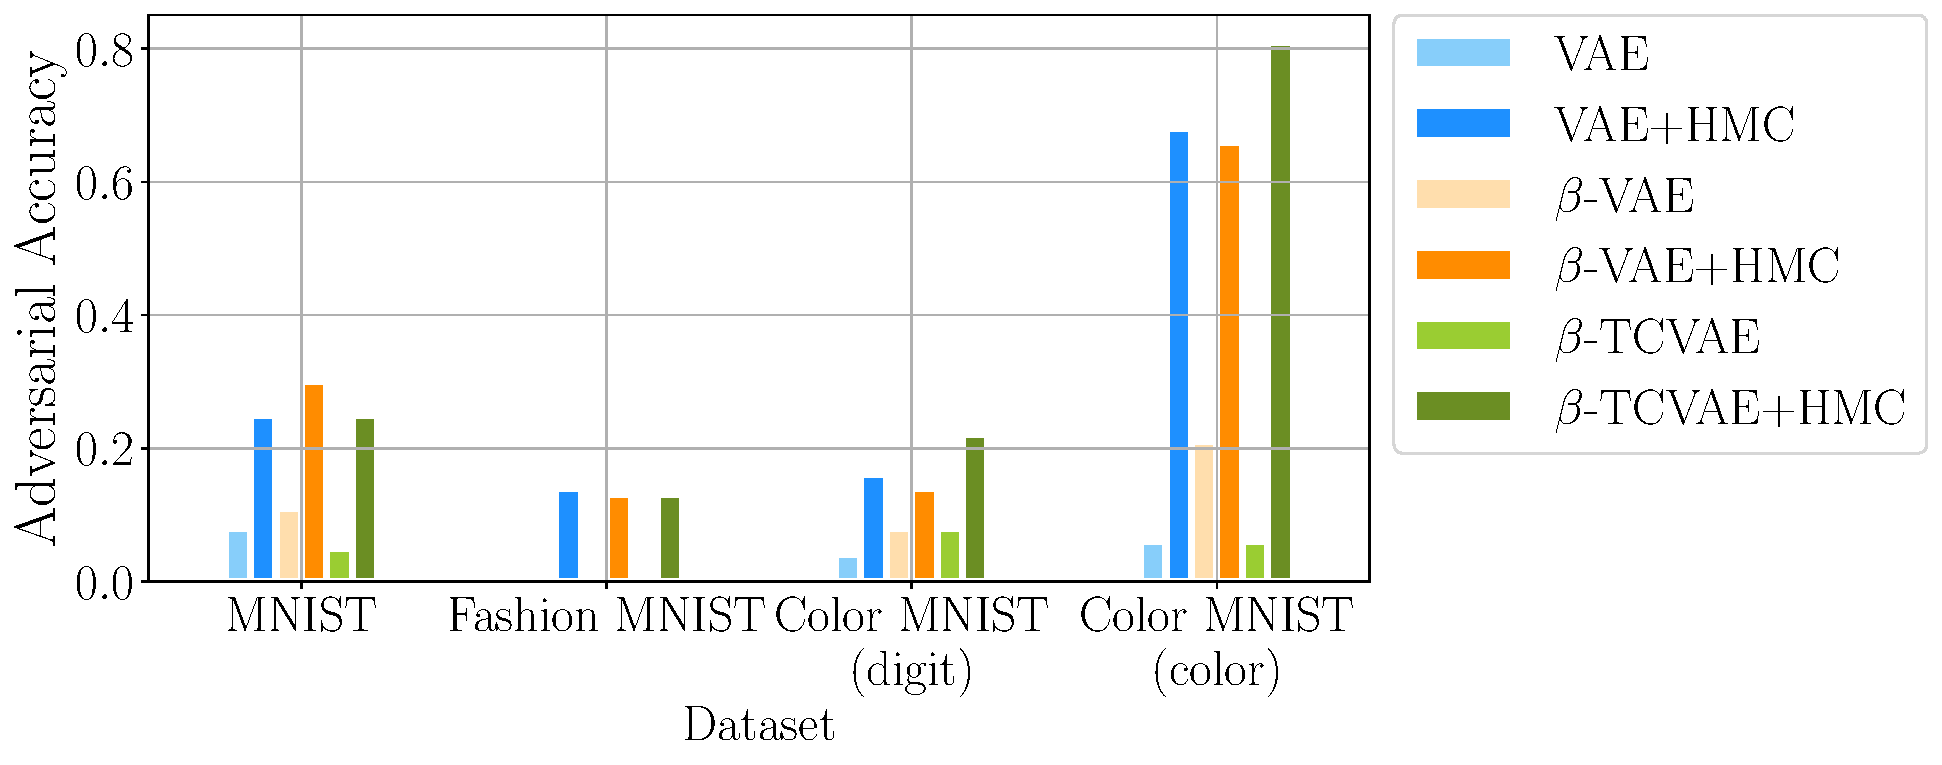
\includegraphics[width=0.5\textwidth]{img/adv_acc_eps_1.pdf} &
%         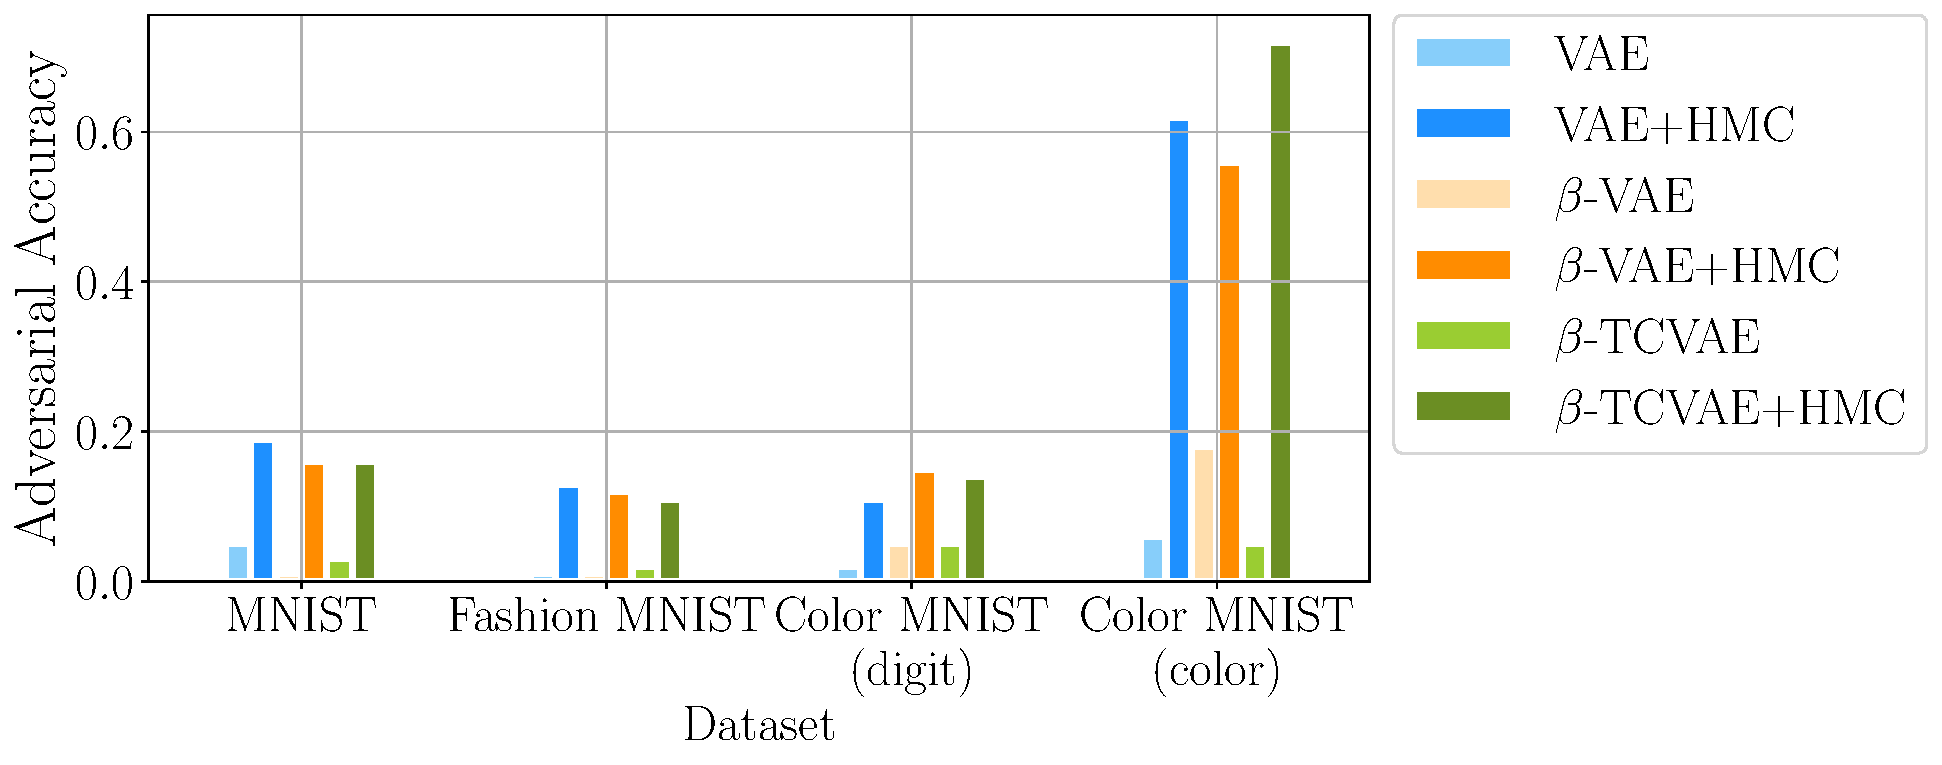
\includegraphics[width=0.5\textwidth]{img/adv_acc_eps_2.pdf} \\
%         \multicolumn{1}{c}{(a) $||\varepsilon ||_{\inf} = 0.1$} &
%         \multicolumn{1}{c}{(b) $||\varepsilon ||_{\inf} = 0.2$} \\
%         % (a) & (b) \\
%         % (c) & (d)
%     \end{tabular}
%     % \vskip -10pt
%     \caption{Improvement of the Adversarial Accuracy after proposed defence. We fix the attack radius to be equal to (a) 0.1 and (b) 0.2.}
%     \vskip -10pt
%     \label{fig:mnist_adv_acc}
% \end{figure}
\paragraph{Attacks on the Encoder} 
In the first setup, we assume that the attacker has access to the encoder of the model $\Enc{z}{x}$ {\cite{barrett2021certifiably, Gondim-Ribeiro2018-cu, Willetts2019-mu}. We use the projected gradient descent (PGD) with 50 steps to maximize the symmetric KL-divergence in the unsupervised setting (\eqref{eq:objective_unsup}). We train 10 adversarial attacks (with different random initialization) for each of 50 reference points. See Appendix \ref{appendix:vae_attack} for the details. We report similarity between the reconstruction of the adversarial and reference point as a measure of the robustness (see Section \ref{sect:adversarial_attacks}). 

\paragraph{Attacks on the downstream task} 
In this setup, we examine how the proposed approach can aleviate the effect of the attack on the downstream tasks in the latent space. For this purpose, we follow the procedure from \cite{cemgil2020autoencoding, Cemgil2019-vn}. Once the VAE is trained, we learn a linear classifier using the mean mappings as features. For the MNIST and Fashion MNIST datasets, we have the 10-class classification problem (digits in the former and pieces of clothing in the latter case). For the ColorMNIST dataset, we consider two classification tasks: the digit classification (10 classes), and the color classification (7 classes). We construct the attack to fool the classifier. See Appendix \ref{appendix:vae_attack} for the details.


\paragraph{Results} 
In Tables \ref{tab:mnist_attack_result} and \ref{tab:color_mnist_attack_results}, we compare our method (VAE + HMC) with the vanilla VAE with other methods in the literature. We report more results and the extended comparison in the Appendix \ref{appendix:beta_vae} where we show that our method combined with $\beta$-VAE and $\beta$-TCVAE leads to the increased robustness. For MNIST and Fashion MNIST (Table \ref{tab:mnist_attack_result}), we observe that the vanilla VAE with the HMC is more robust than $\beta$-VAE and $\beta$-TCVAE. The latter model was shown to be more robust to the latent space attack \cite{Willetts2019-mu}. Still, in our experiments (on different datasets), we could not observe the consistent improvement over the vanilla VAE, when using it with a single level of latent variables. 

In Table \ref{tab:color_mnist_attack_results} we report the result on the ColorMNIST dataset. Here, we additionally compare the adversarial accuracy for our method with the Smooth Encoders (SE) and Autoencoding Variational Autoencoder (AVAE) methods \cite{cemgil2020autoencoding, Cemgil2019-vn}.
% We notice that these methods provide higher adversarial accuracy. However, we have also observed a large discrepancy in terms of the MSE and FID scores of the model itself compared to our experiments, which we suspect might be a result of a mistake in \cite{cemgil2020autoencoding, Cemgil2019-vn}.
% \footnote{We have gotten in touch with the authors, who are kindly working with us to address this issue}

Lastly, we would like to highlight that our defence strategy can be also combined with all the above VAE modifications. One advantage of our approach is that it does not require changing the training procedure of a VAE and, as a result, it does not decrease the quality of the generated images. 
Moreover, we can apply the same procedure to reconstruct the non-corrupted points and it will improve the reconstruction error. 
This result can be seen in the Tables \ref{tab:mnist_attack_result} and \ref{tab:color_mnist_attack_results} and it goes in line with the results of the \cite{salimans2015markov}, where MCMC was used to improve the VAE performance. 
% SE and AVAE methods without any restrictions.  
% Another advantage of our approach is that it does not require changing the training procedure of a VAE and, as a result, it does not decrease the quality of the generated images. \ak{As we observe from the columns \textbf{MSE} and \textbf{FID}, the quality of the vanilla VAE is always better compared to the models with modified training objectives. MODIFY: Mention bridging the gap paper.} We depict several examples of the reconstructions of the attacked point in Figure \ref{fig:adversarial_examples}.


% In Figure \ref{fig:mnist_rec_similarity}, we show how similarity between the reconstructions of the reference and adversarial points increases after the proposed defence is applied. This metric consistently improves for all the datasets, radii and models considered. In Figure \ref{fig:adversarial_examples}, we plot examples for each of the datasets considered (see subsection \ref{sec:nvae} for more details on CelebA experiments). The first two columns contain reference points and their reconstructions (columns a \& b). Then we plot the adversarial input (column c) and its reconstruction without the defence (column d). Finally, we provide the reconstruction with the defence applied (column e) that is much closer to the reconstruction of the reference point.
 


% ==== SubSECTION ====
\begin{figure}[t]
    % \centering
    \begin{adjustbox}{center}
    \begin{tabular}{llll}
        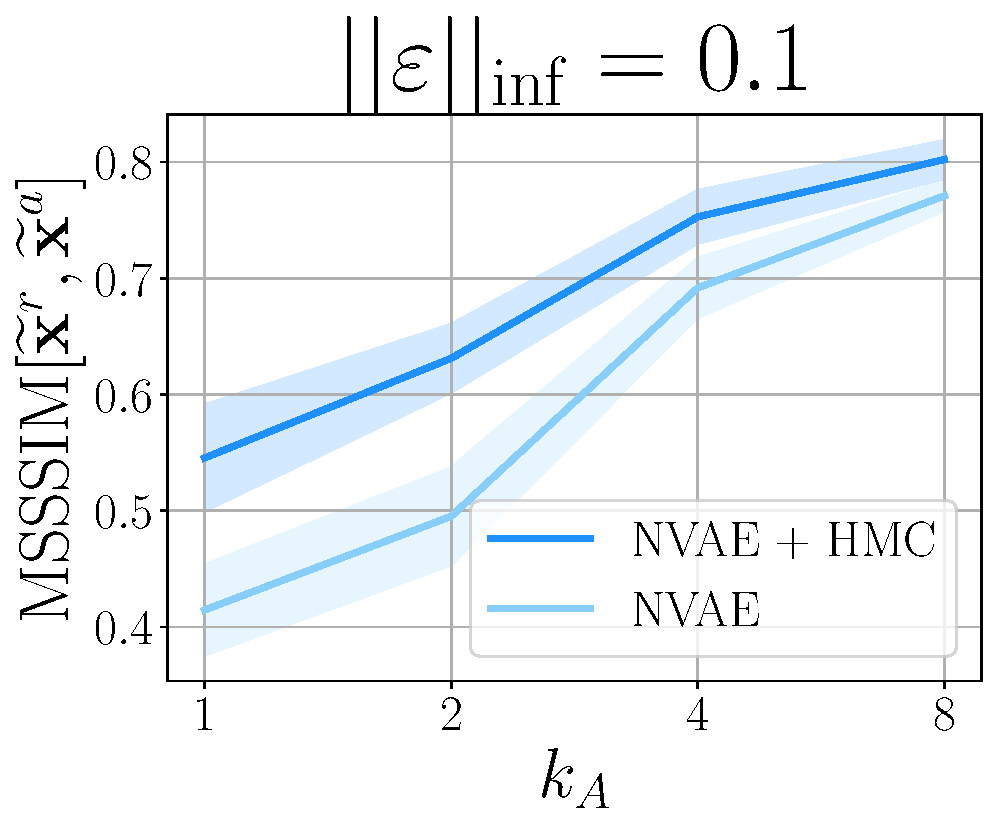
\includegraphics[width=0.4\textwidth]{pics/3_adv_att/nvae_mnist_eps_1.pdf} & 
        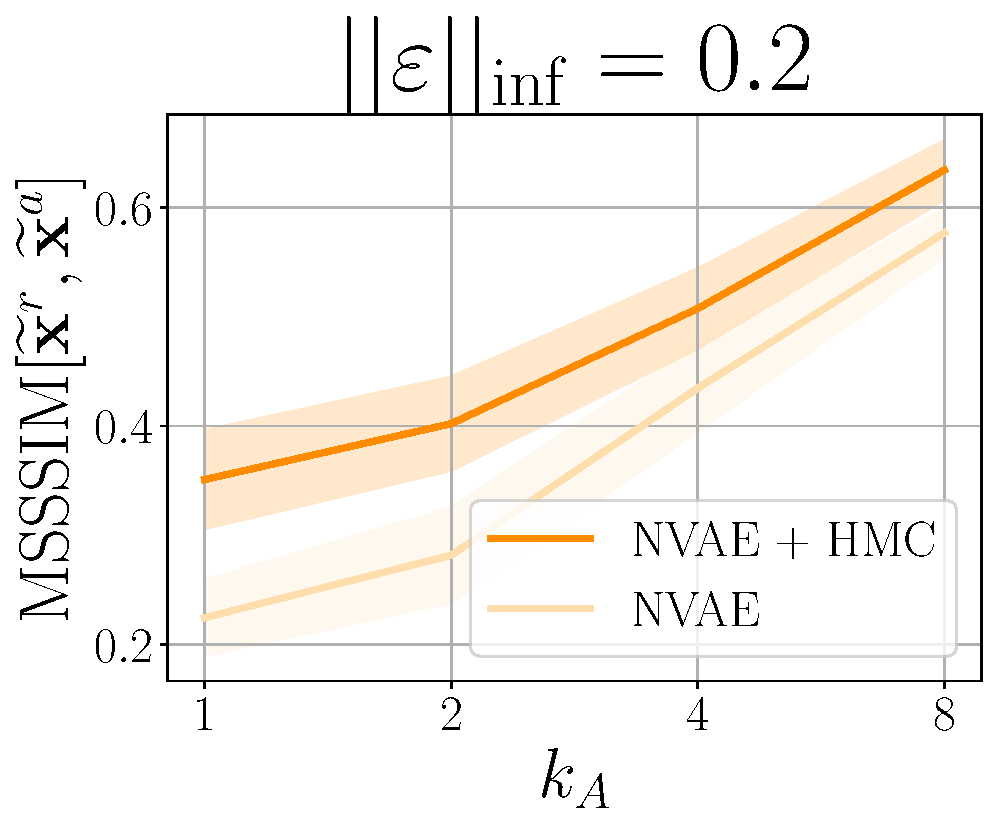
\includegraphics[width=0.4\textwidth]{pics/3_adv_att/nvae_mnist_eps_2.pdf} \\
        \multicolumn{2}{c}{\small (a) The reconstruction similarity for MNIST} \\ \\
        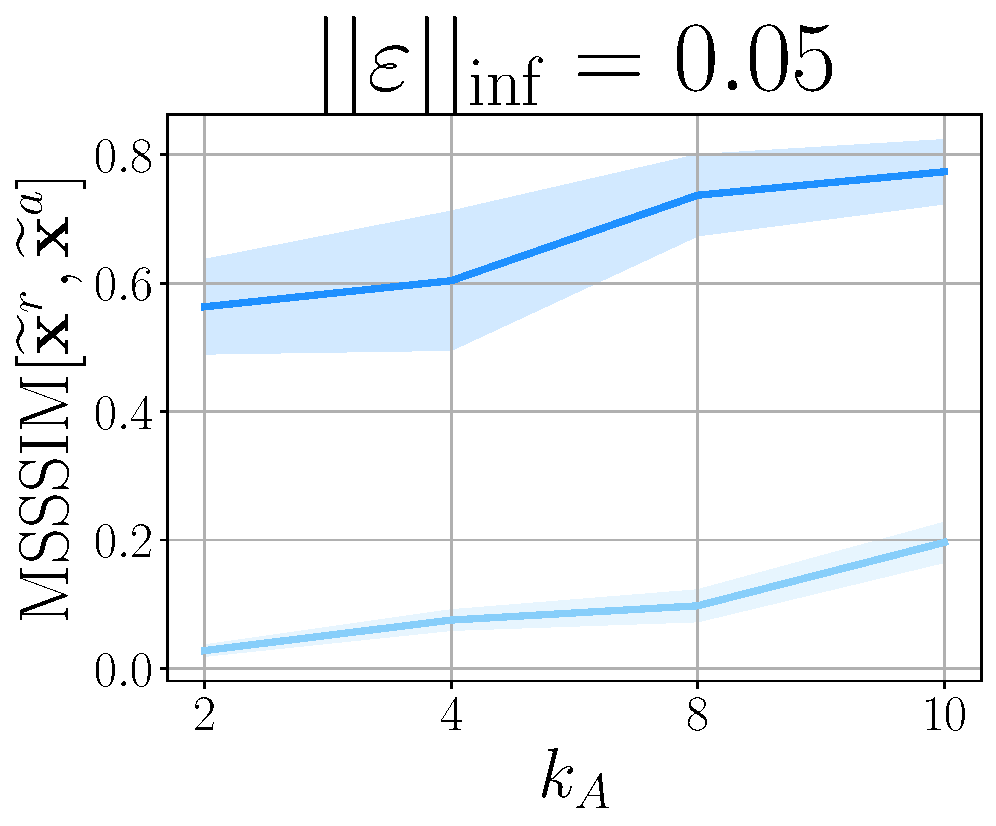
\includegraphics[width=0.4\textwidth]{pics/3_adv_att/nvae_celeba_eps_1.pdf} & 
        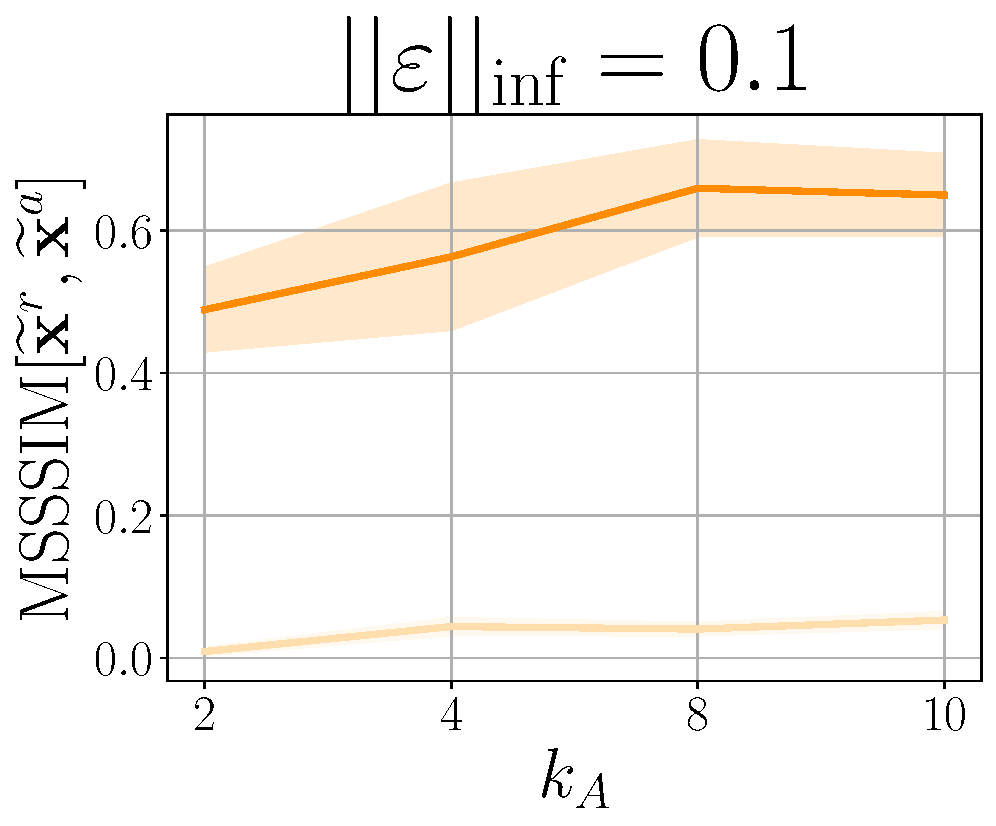
\includegraphics[width=0.4\textwidth]{pics/3_adv_att/nvae_celeba_eps_2.pdf}\\
         \multicolumn{2}{c}{\small (b) The reconstruction similarity for CelebA}\\
    \end{tabular}
    \end{adjustbox}
    \caption[][\baselineskip]{The robustness improvement for the hierarchical model (NVAE) on (a) MNIST and (b) CelebA for two different attack radii. Higher values correspond to more robust representations.}
    \label{fig:nvae_res}
\end{figure}

\subsection{Hierarchical VAE: NVAE}\label{sec:nvae}

\paragraph{Model and datasets} In this section, we explore the robustness of the deep hierarchical VAE (NVAE) \cite{Vahdat2020-xe}, a specific implementation of a hierarchical VAE that works well for high-dimensional data. We attack models trained on MNIST and CelebA \cite{liu2015faceattributes} datasets. We use the weights of the pre-trained model provided in the official NVAE implementation\footnote{The code and model weights were taken from \url{github.com/NVlabs/NVAE}}. 

\paragraph{Attacks construction}
Following \cite{kuzina2021adv} we construct adversarial attacks on the hierarchical VAE by considering higher-level latent variables. That being said, we use latent variables $\{\rvz_{L-k_A}, \rvz_{L-k_A+1}, \dots, \rvz_L\}$ when constructing an attack (\eqref{eq:objective_unsup}). Otherwise, we follow the same procedure we used for VAEs with a single level of latent variables. We assume that the attacker has access to the model's encoder and uses the symmetric KL-divergence as the objective. The radius of an attack is measured with the $L_{\inf}$ norm. For optimization, we use the projected gradient descent with the number of iterations limited to 50 per point. Further details are reported in the Appendix \ref{appendix:vae_attack}.


\paragraph{Results}
In Figure \ref{fig:nvae_res}, we present reconstruction similarity of the reference and adversarial points for both datasets. We observe that the proposed method consistently improves the robustness of the model to the adversarial attack. This result is in line with our theoretical considerations where a flexible class of variational posteriors could help to counteract adversarial attacks and, eventually, deacrease the bias of the class of models measured in terms of the KL-divergence. Additionally, applying the MCMC can further help us to counteract the attack. In Figure \ref{fig:adversarial_examples} (the two bottom rows), we show how an adversarial point (c) is reconstructed without any defence (d) and with the proposed defence (e). In the depicted samples, we have used the top 10 latent variables ($k_A = 10$) to construct the attack with a radius of 0.05. 



% \begin{wrapfigure}{r}{0.62\textwidth}
\begin{figure}[t]
    \centering
    \begin{tabular}{cc}
     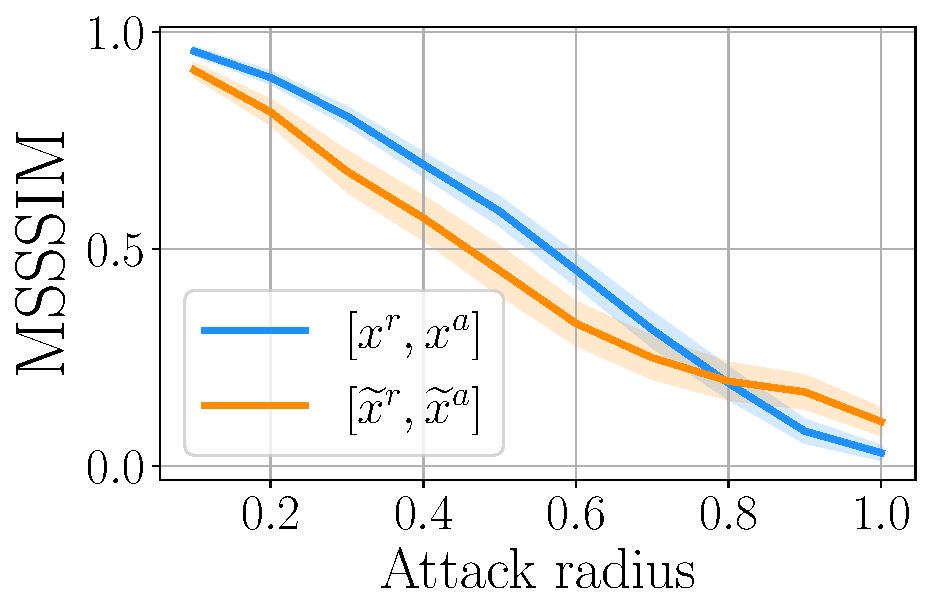
\includegraphics[width=0.4\linewidth]{pics/3_adv_att/attack_mcmc_0_100.pdf} &
     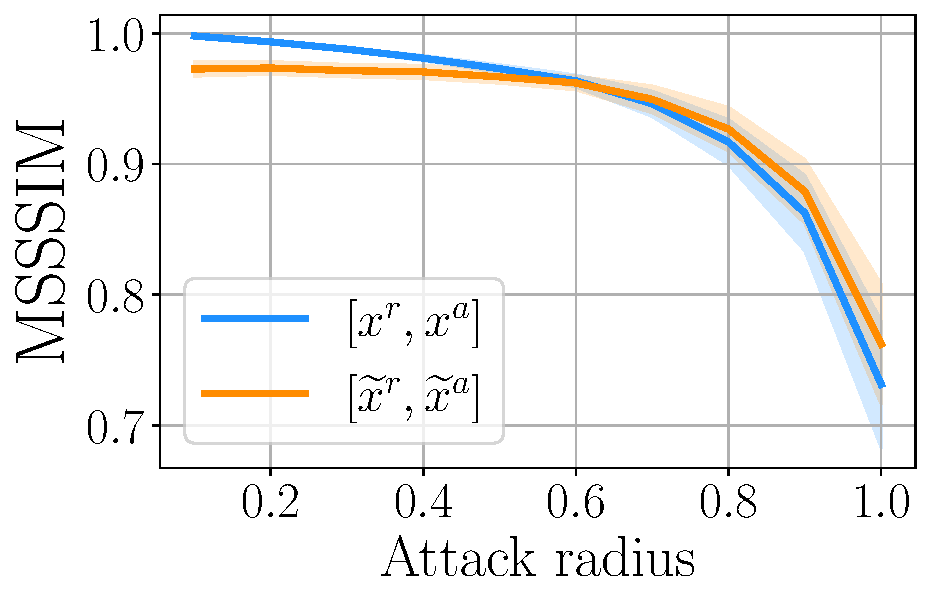
\includegraphics[width=0.4\linewidth]{pics/3_adv_att/attack_mcmc_1_100.pdf} \\
     \multirow{2}{0.45\linewidth}{\centering \small (a) An attacker does not know the defence strategy}&
     \multirow{2}{0.45\linewidth}{\centering \small (b) An attacker knows the defence strategy }\\
     \\
    \end{tabular}
    \caption{Robustness to adversarial attack (with HMC defence). We report similarity of the reference and adversarial point (blue) and their reconstructions (orange).}
    \label{fig:attack_mcmc}
	\vspace*{\baselineskip}
\end{figure}

% \end{wrapfigure}


\subsection{Ablation Study: What if the attacker knows the defence strategy?} \label{sec:ablation}
In our experiments, we rely on the assumption that the attacker does not take into account the defence strategy that we use. We believe that it is reasonable, since the defence requires access to the decoder part of the model, $p_{\theta}(x|z)$, which is not necessarily available to the attacker. 

In this ablation study we verify how the robustness results change if we construct the attack with the access to the defence strategy. We train an adversarial attack with the modified objective \ref{eq:objective_unsup}, which takes into account the HMC step. See Appendix \ref{appendix:attack_mcmc} for more details on the experimental setup. 

In Figure \ref{fig:attack_mcmc} we show the experiment results for various attack radii between 0 and 1. We observe that constructing an attack with such an objective is much harder (Figure \ref{fig:attack_mcmc} (b)).  

% In both cases the reconstructions are almost as close as the initial points, which proves the defence strategy to be successful for this experiment.

% Here we consider the most straightforward approach to construct an attack, which is aligned with the previous works on attacking VAEs. 

% It is, however, possible to use more sophisticated adaptive methods \cite{tramer2020adaptive, athalye2018obfuscated}. We are not aware of the works where such attacks were applied to VAEs and believe that it is an interesting direction for the future work on the topic. 


% \ak{add reference to papers with MCMC defence and attacks, explain that it is out of scope of this paper.}
% In Appendix \ref{appendix:attack_mcmc} we report results of the ablation study, where attacks on the encoder are constructed assuming that the attacker knows the defence strategy and attempts to use it during the attack construction. We observe that using MCMC during the attack construction does not help the attacker. On the contrary, it becomes harder to find a reasonable additive perturbation of the input.





\section{Discussion}
Following the previous works on attacking VAEs \cite{barrett2021certifiably, camuto2021towards, cemgil2020autoencoding, Cemgil2019-vn, Gondim-Ribeiro2018-cu, Willetts2019-mu}, we only consider the projected gradient descent as a way to construct the attack. However, more sophisticated adaptive methods \cite{ athalye2018obfuscated, tramer2020adaptive} were proposed to attack discriminative model and can be potentially applied to VAEs as well.
% We are not aware of the works where such attacks were applied to VAEs and 
We believe that it is an interesting direction for the future work. 

\paragraph{Objective Function}
For the unsupervised attack on the encoder, we use the symmetric KL-divergence to measure the dissimilarity. However, other options are possible, e.g., the forward or reverse KL-divergence or even $L_2$ distance between the means (see Table \ref{tab:attack_variation}). In our comparative experiments (see Appendix \ref{appendix:objectives}), we observe that no single objective consistently performs better than others.

% \paragraph{What if attacker knows the defence strategy?}
% In Appendix \ref{appendix:attack_mcmc} we report results of the ablation study, where attacks on the encoder are constructed assuming that the attacker knows the defence strategy and attempts to use it during the attack construction. We observe that using MCMC during the attack construction does not help the attacker. On the contrary, it becomes harder to find a reasonable additive perturbation of the input.

\paragraph{Attack radius}
During the attack construction we seek to obtain a point that will have the most different latent representation or a different predicted class. However, it is also important that the point itself is as similar to the initial reference point as possible. In Appendix \ref{appendix:attack_radius}, we visualize how the attacks of different radii influence the similarity between the adversarial and reference points. Based on these results, we have chosen the radii which do not allow adversarial points to deviate a lot from the reference (as measured by \textsc{MSSSIM}): $\|\varepsilon\|_{\inf} \leq 0.2$ for the MNIST dataset (which goes in line with the previous works \cite{cemgil2020autoencoding, Cemgil2019-vn}) and $\|\varepsilon\|_{\inf} \leq 0.1$ for the CelebA dataset. 


%\begin{wrapfigure}{r}{0.54\textwidth}
%\vskip -10pt
%    % \centering
%    \begin{tabular}{c}
%        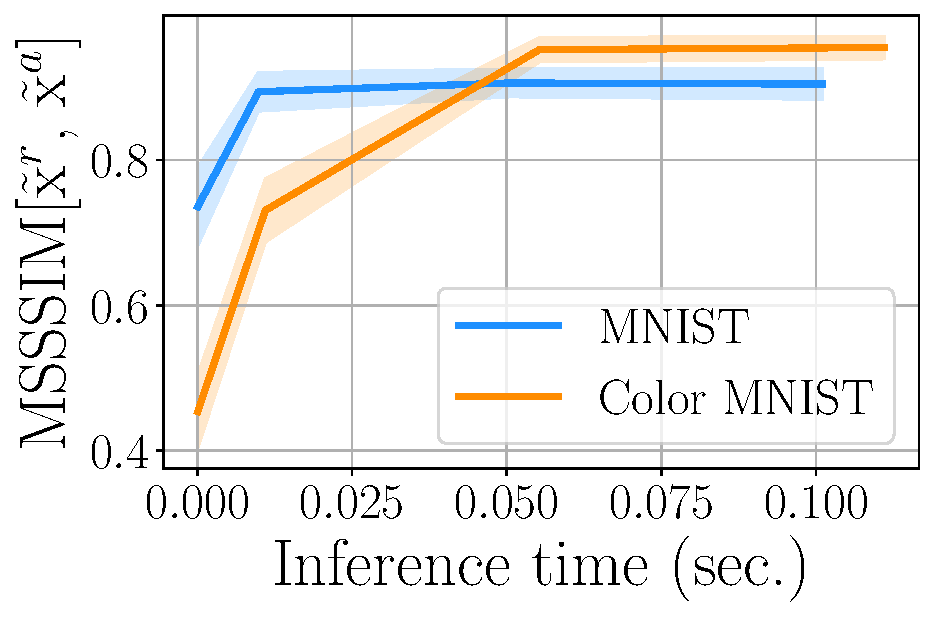
\includegraphics[width=0.8\linewidth]{pics/3_adv_att/hmc_steps_time_ref_rec_sim.pdf} \\
%        % \includegraphics[width=\linewidth]{img/hmc_steps_time_adv_acc.pdf} \\ 
%    \end{tabular}
%    \vskip -5pt
%    \caption{Trade-off between robustness and inference time.}
%    \label{fig:time_vs_performance}
%\end{wrapfigure}


\paragraph{Number of MCMC steps and Inference Time}
In our approach, we have to select the number of MCMC steps that the defender performs. This parameter potentially can be critical as it influences both the inference time (see Appendix \ref{appendix:inference_time}) and the performance (see Appendix \ref{appendix:hmc_steps}). 
In Figure \ref{fig:time_vs_performance} we show the trade-off between the reconstruction similarity and the inference time. The increase in the inference time is cause by a larger number of HMC steps used (we consider 0, 100, 500 and 1000 steps for this experiment).
\begin{marginfigure}
	\vspace*{-8\baselineskip}
	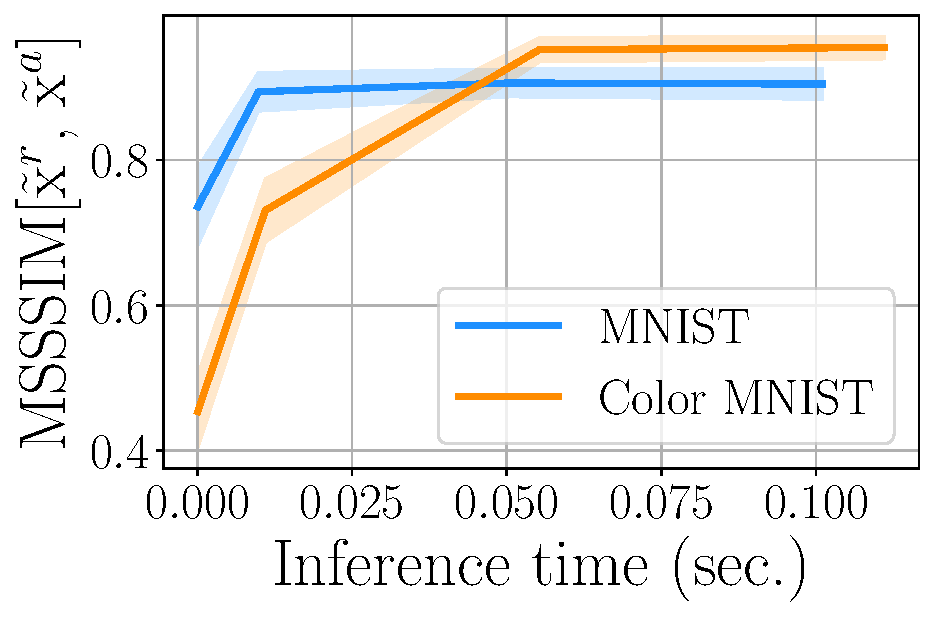
\includegraphics[width=\linewidth]{pics/3_adv_att/hmc_steps_time_ref_rec_sim.pdf} 
	\caption{Trade-off between robustness and inference time.}
	\label{fig:time_vs_performance}
\end{marginfigure}

% In our approach, we have to select the number of MCMC steps that the defender performs. This parameter potentially can be critical \upd{as it influences the inference time (see Appendix \ref{appendix:inference_time}}. Following the theoretical analysis, the more steps in the MCMC procedure is taken, the tighter the bound (\ref{eq:theorem_1_main}) is. On the other hand, typically we have time and computational constraints to take into account. In Appendix \ref{appendix:hmc_steps}, we show the method's performance for the number of HMC steps ranging between 0 and 2000. There is a considerable jump in robustness between 0 and 100 steps. At the same time, we do not observe much improvement as we continue to increase the number of steps. 

\section{Conclusion}
In this work, we explore the robustness of VAEs to adversarial attacks.  We propose a theoretically justified method that allows alleviating the effect of attacks on the latent representations by improving the reconstructions of the adversarial inputs and the downstream tasks accuracy. We experimentally validate our approach on a variety of datasets: both grey-scale (MNIST, Fashion MNIST) and colored (ColorMNIST, CelebA) data. We show that the proposed method improves the robustness of the vanilla VAE models and its various modifications, i.e., $\beta$-VAE, $\beta$-TCVAE and NVAE.

